\documentclass[aspectratio=169,professionalfonts]{beamer}
\usepackage[utf8]{inputenc}
\usepackage[T1]{fontenc}
\usepackage{lmodern}
\usepackage{amsmath,amssymb,mathtools}
\usepackage{booktabs}
\usepackage{array}
\usepackage{multirow}
\usepackage{tikz}
\usetikzlibrary{matrix,positioning,fit,calc,backgrounds,decorations.pathreplacing,arrows.meta}
\usepackage{microtype}

\usetheme{Madrid}
\usecolortheme{default}
\setbeamertemplate{navigation symbols}{}
\setbeamertemplate{footline}[frame number]
\setbeamertemplate{blocks}[rounded][shadow=false]
\setbeamerfont{frametitle}{series=\bfseries,size=\large}
\setbeamerfont{title}{series=\bfseries}
\setbeamercolor{structure}{fg=blue!55!black}
\setbeamercolor{frametitle}{fg=blue!55!black}
\setbeamercolor{title}{fg=blue!55!black}
\setbeamercolor{block title}{bg=blue!8,fg=blue!55!black}
\setbeamercolor{block body}{bg=blue!2,fg=black}
\setbeamertemplate{itemize item}{\color{blue!55!black}$\blacktriangleright$}
\setbeamertemplate{itemize subitem}{\color{blue!55!black}$\triangleright$}

\newcommand{\Oh}{\mathcal{O}}
\newcommand{\fd}{f_d}
\newcommand{\cK}{\mathcal{K}}
\newcommand{\cR}{\mathcal{R}}
\newcommand{\cP}{\mathcal{P}}
\newcommand{\cQ}{\mathcal{Q}}
\newcommand{\cO}{\mathcal{O}}
\newcommand{\cC}{\mathcal{C}}
\newcommand{\cA}{\mathcal{A}}
\newcommand{\cB}{\mathcal{B}}
\newcommand{\strips}{\mathtt{strips}}
\newcommand{\slabstart}{\mathsf{slab_start}}
\newcommand{\bbS}{\mathbb{S}}
\newcommand{\bbP}{\mathbb{P}}
\newcommand{\bbQ}{\mathbb{Q}}
\newcommand{\bbA}{\mathbb{A}}
\newcommand{\bbW}{\mathbb{W}}
\newcommand{\bbD}{\mathbb{D}}
\newcommand{\blank}{\perp}
\newcommand{\Seg}[1]{[#1]}

\tikzset{
mat/.style={matrix of nodes,nodes in empty cells,
nodes={draw=black!55,minimum width=4.9mm,minimum height=4.9mm,inner sep=0pt,font=\scriptsize},
row sep=-\pgflinewidth,column sep=-\pgflinewidth,ampersand replacement=\&,anchor=center},
mini/.style={matrix of nodes,nodes in empty cells,
nodes={draw=black!55,minimum width=4.0mm,minimum height=4.0mm,inner sep=0pt,font=\tiny},
row sep=-\pgflinewidth,column sep=-\pgflinewidth,ampersand replacement=\&,anchor=center},
zero/.style={fill=white},
one/.style={fill=blue!7},
slabA/.style={fill=blue!18},
slabB/.style={fill=orange!28},
slabC/.style={fill=green!22},
slabD/.style={fill=red!18},
slabE/.style={fill=gray!25},
slabF/.style={fill=yellow!35},
slabG/.style={fill=cyan!20},
slabH/.style={fill=violet!18},
update0/.style={fill=red!35,font=\scriptsize\bfseries},
update1/.style={fill=green!35,font=\scriptsize\bfseries},
corner/.style={fill=magenta!22},
zoneframe/.style={draw=blue!70!black,very thick,rounded corners=1pt},
softframe/.style={draw=black!55,thick,rounded corners=1pt},
segline/.style={line width=3pt,blue!55!black},
seglineb/.style={line width=3pt,orange!80!black},
faintseg/.style={line width=2.8pt,black!20},
tick/.style={black!70,line width=0.45pt},
explain/.style={font=\scriptsize,align=left},
tinyexplain/.style={font=\tiny,align=left},
timeline/.style={draw=black!55,rounded corners=2pt,minimum height=5mm,inner sep=2pt,font=\scriptsize,align=center},
flowarrow/.style={-{Latex[length=2mm,width=1.5mm]},very thick,blue!55!black}
}

\newcommand{\Zero}[1]{|[zero]| #1}
\newcommand{\One}[1]{|[one]| #1}
\newcommand{\Acell}[1]{|[slabA]| #1}
\newcommand{\Bcell}[1]{|[slabB]| #1}
\newcommand{\Ccell}[1]{|[slabC]| #1}
\newcommand{\Dcell}[1]{|[slabD]| #1}
\newcommand{\Ecell}[1]{|[slabE]| #1}
\newcommand{\Fcell}[1]{|[slabF]| #1}
\newcommand{\Gcell}[1]{|[slabG]| #1}
\newcommand{\Hcell}[1]{|[slabH]| #1}
\newcommand{\UpdZero}{|[update0]| 0}
\newcommand{\UpdOne}{|[update1]| 1}
\newcommand{\CornerCell}[1]{|[corner]| #1}

% --- reusable matrix figures ---
\newcommand{\ContractionStateOne}[1][1]{%
\begin{tikzpicture}[scale=#1,every node/.style={transform shape}]
\matrix[mini] (m) {
\Zero{0} \& \One{1} \& \One{1} \& \One{1} \& \One{1}\\
\Zero{0} \& \Zero{0} \& \Zero{0} \& \Zero{0} \& \One{1}\\
\One{1} \& \One{1} \& \One{1} \& \Zero{0} \& \Zero{0}\\
\One{1} \& \One{1} \& \One{1} \& \Zero{0} \& \One{1}\\
\One{1} \& \Zero{0} \& \Zero{0} \& \One{1} \& \One{1}\\
};
\end{tikzpicture}}

\newcommand{\ContractionStateTwo}[1][1]{%
\begin{tikzpicture}[scale=#1,every node/.style={transform shape}]
\matrix[mini] (m) {
\Zero{0} \& \One{1} \& \One{1} \& \One{1} \& \One{1}\\
\Zero{0} \& \Zero{0} \& \Zero{0} \& \Zero{0} \& \One{1}\\
\One{1} \& \One{1} \& \One{1} \& \Zero{0} \& \Acell{0}\\
\One{1} \& \One{1} \& \One{1} \& \Zero{0} \& \Acell{1}\\
\One{1} \& \Zero{0} \& \Zero{0} \& \One{1} \& \One{1}\\
};
\draw[white,line width=1.2pt] ($(m-3-1.south west)+(0,0.02)$) -- ($(m-3-5.south east)+(0,0.02)$);
\end{tikzpicture}}

\newcommand{\ContractionStateThree}[1][1]{%
\begin{tikzpicture}[scale=#1,every node/.style={transform shape}]
\matrix[mini] (m) {
\Zero{0} \& \One{1} \& \One{1} \& \One{1} \& \One{1}\\
\Zero{0} \& \Zero{0} \& \Zero{0} \& \Zero{0} \& \One{1}\\
\One{1} \& \One{1} \& \One{1} \& \Zero{0} \& \Acell{0}\\
\One{1} \& \One{1} \& \One{1} \& \Zero{0} \& \Acell{1}\\
\One{1} \& \Zero{0} \& \Zero{0} \& \One{1} \& \One{1}\\
};
\draw[white,line width=1.2pt] ($(m-3-1.south west)+(0,0.02)$) -- ($(m-3-5.south east)+(0,0.02)$);
\draw[white,line width=1.2pt] ($(m-1-2.north east)+(-0.02,0)$) -- ($(m-5-2.south east)+(-0.02,0)$);
\end{tikzpicture}}

\newcommand{\ContractionStateFour}[1][1]{%
\begin{tikzpicture}[scale=#1,every node/.style={transform shape}]
\matrix[mini] (m) {
\Zero{0} \& \Bcell{1} \& \Bcell{1} \& \Bcell{1} \& \One{1}\\
\Zero{0} \& \Bcell{0} \& \Bcell{0} \& \Bcell{0} \& \One{1}\\
\One{1} \& \One{1} \& \One{1} \& \Zero{0} \& \Acell{0}\\
\One{1} \& \One{1} \& \One{1} \& \Zero{0} \& \Acell{1}\\
\One{1} \& \Zero{0} \& \Zero{0} \& \One{1} \& \One{1}\\
};
\draw[white,line width=1.2pt] ($(m-1-1.south west)+(0,0.02)$) -- ($(m-1-5.south east)+(0,0.02)$);
\draw[white,line width=1.2pt] ($(m-3-1.south west)+(0,0.02)$) -- ($(m-3-5.south east)+(0,0.02)$);
\draw[white,line width=1.2pt] ($(m-1-2.north east)+(-0.02,0)$) -- ($(m-5-2.south east)+(-0.02,0)$);
\end{tikzpicture}}

\newcommand{\ContractionStateFive}[1][1]{%
\begin{tikzpicture}[scale=#1,every node/.style={transform shape}]
\matrix[mini] (m) {
\Zero{0} \& \Bcell{1} \& \Bcell{1} \& \Ccell{1} \& \Ccell{1}\\
\Zero{0} \& \Bcell{0} \& \Bcell{0} \& \Ccell{0} \& \Ccell{1}\\
\One{1} \& \One{1} \& \One{1} \& \Acell{0} \& \Acell{0}\\
\One{1} \& \One{1} \& \One{1} \& \Acell{0} \& \Acell{1}\\
\One{1} \& \Zero{0} \& \Zero{0} \& \One{1} \& \One{1}\\
};
\draw[white,line width=1.2pt] ($(m-1-1.south west)+(0,0.02)$) -- ($(m-1-5.south east)+(0,0.02)$);
\draw[white,line width=1.2pt] ($(m-3-1.south west)+(0,0.02)$) -- ($(m-3-5.south east)+(0,0.02)$);
\draw[white,line width=1.2pt] ($(m-1-2.north east)+(-0.02,0)$) -- ($(m-5-2.south east)+(-0.02,0)$);
\draw[white,line width=1.2pt] ($(m-1-4.north west)+(0.02,0)$) -- ($(m-5-4.south west)+(0.02,0)$);
\end{tikzpicture}}

\newcommand{\ContractionStateSix}[1][1]{%
\begin{tikzpicture}[scale=#1,every node/.style={transform shape}]
\matrix[mini] (m) {
\Bcell{0} \& \Bcell{1} \& \Bcell{1} \& \Ccell{1} \& \Ccell{1}\\
\Bcell{0} \& \Bcell{0} \& \Bcell{0} \& \Ccell{0} \& \Ccell{1}\\
\Dcell{1} \& \Dcell{1} \& \Dcell{1} \& \Acell{0} \& \Acell{0}\\
\Dcell{1} \& \Dcell{1} \& \Dcell{1} \& \Acell{0} \& \Acell{1}\\
\Ecell{1} \& \Ecell{0} \& \Ecell{0} \& \One{1} \& \One{1}\\
};
\draw[white,line width=1.2pt] ($(m-3-1.south west)+(0,0.02)$) -- ($(m-3-5.south east)+(0,0.02)$);
\draw[white,line width=1.2pt] ($(m-1-4.north west)+(0.02,0)$) -- ($(m-5-4.south west)+(0.02,0)$);
\end{tikzpicture}}

\newcommand{\PrelimSlabFig}[1][1]{%
\begin{tikzpicture}[scale=#1,every node/.style={transform shape}]
\matrix[mat] (m) {
\Zero{0} \& \Bcell{1} \& \Bcell{1} \& \Zero{0} \& \Ecell{1}\\
\Zero{0} \& \Zero{0} \& \Zero{0} \& \Zero{0} \& \Ecell{1}\\
\Zero{0} \& \Ccell{1} \& \Ccell{1} \& \Ccell{1} \& \Zero{0}\\
\Acell{1} \& \Acell{1} \& \Acell{1} \& \Zero{0} \& \Dcell{1}\\
\Acell{1} \& \Acell{1} \& \Acell{1} \& \Zero{0} \& \Dcell{1}\\
};
\end{tikzpicture}}

\newcommand{\ZoneCornerSlabFig}[1][1]{%
\begin{tikzpicture}[scale=#1,every node/.style={transform shape}]
\matrix[mat] (m) {
\Zero{0} \& \Bcell{1} \& \Bcell{1} \& \Zero{0} \& \Ecell{1}\\
\Zero{0} \& \Zero{0} \& \Zero{0} \& \Zero{0} \& \Ecell{1}\\
\Zero{0} \& \Ccell{1} \& \Ccell{1} \& \Ccell{1} \& \Zero{0}\\
\Acell{1} \& \Acell{1} \& \CornerCell{1} \& \CornerCell{0} \& \Dcell{1}\\
\Acell{1} \& \Acell{1} \& \CornerCell{1} \& \CornerCell{0} \& \Dcell{1}\\
};
\node[zoneframe,fit=(m-3-2)(m-3-4)] {};
\node[softframe,fit=(m-4-1)(m-5-3)] {};
\end{tikzpicture}}

\newcommand{\CanonicalExampleOne}[1][1]{%
\begin{tikzpicture}[scale=#1,every node/.style={transform shape}]
\matrix[mat] (m) {
\Ccell{1} \& \Ecell{1} \& \Acell{1} \& \Dcell{1} \& \Dcell{1}\\
\Zero{0} \& \Ecell{1} \& \Zero{0} \& \Dcell{1} \& \Dcell{1}\\
\Hcell{1} \& \Ecell{1} \& \Zero{0} \& \Zero{0} \& \Zero{0}\\
\Hcell{1} \& \Ecell{1} \& \Fcell{1} \& \Fcell{1} \& \Fcell{1}\\
\Hcell{1} \& \Zero{0} \& \Zero{0} \& \Zero{0} \& \Zero{0}\\
};
\end{tikzpicture}}

\newcommand{\CanonicalExampleTwo}[1][1]{%
\begin{tikzpicture}[scale=#1,every node/.style={transform shape}]
\matrix[mat] (m) {
\Zero{0} \& \Fcell{1} \& \Fcell{1} \& \Zero{0} \& \Zero{0}\\
\Zero{0} \& \Fcell{1} \& \Fcell{1} \& \Zero{0} \& \Zero{0}\\
\Ecell{1} \& \Fcell{1} \& \Fcell{1} \& \Dcell{1} \& \Zero{0}\\
\Ecell{1} \& \Fcell{1} \& \Fcell{1} \& \Dcell{1} \& \Zero{0}\\
\Zero{0} \& \Zero{0} \& \Zero{0} \& \Zero{0} \& \Zero{0}\\
};
\end{tikzpicture}}

\newcommand{\CanonicalTwoCoarse}[1][1]{%
\begin{tikzpicture}[scale=#1,every node/.style={transform shape}]
\matrix[mat] (m) {
\Zero{0} \& \Bcell{1} \& \Bcell{1} \& \Zero{0} \& \Zero{0}\\
\Zero{0} \& \Bcell{1} \& \Bcell{1} \& \Zero{0} \& \Zero{0}\\
\Acell{1} \& \Acell{1} \& \Acell{1} \& \Acell{1} \& \Zero{0}\\
\Acell{1} \& \Acell{1} \& \Acell{1} \& \Acell{1} \& \Zero{0}\\
\Zero{0} \& \Zero{0} \& \Zero{0} \& \Zero{0} \& \Zero{0}\\
};
\end{tikzpicture}}

\newcommand{\StripsExampleFig}[1][1]{%
\begin{tikzpicture}[scale=#1,every node/.style={transform shape}]
\matrix[mat] (m) {
\Zero{0} \& \Fcell{1} \& \Fcell{1} \& \Zero{0}\\
\Acell{1} \& \Fcell{1} \& \Fcell{1} \& \Zero{0}\\
\Acell{1} \& \Fcell{1} \& \Fcell{1} \& \Dcell{1}\\
\Zero{0} \& \Zero{0} \& \Zero{0} \& \Dcell{1}\\
\Zero{0} \& \Gcell{1} \& \Gcell{1} \& \Dcell{1}\\
};
\draw[blue!80!black,very thick] ($(m-1-2.north west)+(-0.06,0.06)$) rectangle ($(m-3-2.south east)+(0.06,-0.06)$);
\draw[orange!80!black,very thick] ($(m-1-3.north west)+(-0.06,0.06)$) rectangle ($(m-3-3.south east)+(0.06,-0.06)$);
\draw[green!60!black,very thick] ($(m-5-2.north west)+(-0.06,0.06)$) rectangle ($(m-5-3.south east)+(0.06,-0.06)$);
\end{tikzpicture}}

\newcommand{\SweepMatrixFig}[1][1]{%
\begin{tikzpicture}[scale=#1,every node/.style={transform shape}]
\matrix[mat] (m) {
\Zero{0} \& \Zero{0} \& \Zero{0} \& \Ecell{1}\\
\Dcell{1} \& \Dcell{1} \& \Dcell{1} \& \Zero{0}\\
\Zero{0} \& \Fcell{1} \& \Fcell{1} \& \Fcell{1}\\
\Acell{1} \& \Acell{1} \& \Acell{1} \& \Acell{1}\\
};
\end{tikzpicture}}

\newcommand{\AmortizedBaseFig}[1][1]{%
\begin{tikzpicture}[scale=#1,every node/.style={transform shape}]
\matrix[mat] (m) {
\Zero{0} \& \UpdZero \& \Zero{0} \& \Ecell{1} \& \Zero{0}\\
\Zero{0} \& \Zero{0} \& \Zero{0} \& \Ecell{1} \& \Zero{0}\\
\Acell{1} \& \Acell{1} \& \Fcell{1} \& \Zero{0} \& \Zero{0}\\
\Acell{1} \& \Acell{1} \& \Fcell{1} \& \UpdOne \& \Gcell{1}\\
\Acell{1} \& \UpdZero \& \Zero{0} \& \Gcell{1} \& \Gcell{1}\\
};
\end{tikzpicture}}

\newcommand{\AmortizedAfterFig}[1][1]{%
\begin{tikzpicture}[scale=#1,every node/.style={transform shape}]
\matrix[mat] (m) {
\Zero{0} \& \Zero{0} \& \Zero{0} \& \Ecell{1} \& \Zero{0}\\
\Zero{0} \& \Zero{0} \& \Zero{0} \& \Ecell{1} \& \Zero{0}\\
\Acell{1} \& \Bcell{1} \& \Bcell{1} \& \Zero{0} \& \Zero{0}\\
\Acell{1} \& \Bcell{1} \& \Bcell{1} \& \Dcell{1} \& \Dcell{1}\\
\Acell{1} \& \Zero{0} \& \Zero{0} \& \Dcell{1} \& \Dcell{1}\\
};
\end{tikzpicture}}

\newcommand{\PointLocationFig}[1][1]{%
\begin{tikzpicture}[scale=#1,every node/.style={transform shape}]
\draw[fill=gray!6] (0,0) rectangle (4.8,4.8);
\draw[fill=blue!18] (0.6,2.8) rectangle (2.6,4.2);
\draw[fill=orange!28] (2.6,1.6) rectangle (4.2,3.6);
\draw[fill=green!22] (0.8,0.6) rectangle (2.0,2.0);
\draw[fill=red!18] (3.2,0.6) rectangle (4.4,1.4);
\draw[black!60] (0,0) rectangle (4.8,4.8);
\foreach \x/\lab in {0.6/1,1.6/2,2.6/3,3.6/4,4.6/5} {\draw[tick] (\x,0) -- +(0,-0.12); \node[font=\tiny,below] at (\x,0) {\lab};}
\foreach \y/\lab in {0.6/1,1.6/2,2.6/3,3.6/4,4.6/5} {\draw[tick] (0,\y) -- +(-0.12,0); \node[font=\tiny,left] at (0,\y) {\lab};}
\fill[blue!70!black] (3.55,2.35) circle (0.07);
\draw[flowarrow] (3.65,2.45) -- (4.55,4.5);
\node[explain,anchor=west] at (4.62,4.5) {query $(i,j)$};
\node[tinyexplain] at (1.6,3.5) {slab};
\node[tinyexplain] at (3.4,2.6) {slab};
\end{tikzpicture}}

\newcommand{\SegmentExampleOne}[1][1]{%
\begin{tikzpicture}[scale=#1,every node/.style={transform shape}]
\foreach \x in {0,...,8} {\draw[tick] (\x,0.1) -- (\x,-0.1);}
\draw[black!50] (0,0) -- (8,0);
\foreach \x/\lab in {0/1,1/2,2/3,3/4,4/5,5/6,6/7,7/8} {\node[font=\tiny,below] at (\x,-0.12) {\lab};}
\draw[segline] (1,0) -- (2,0);
\draw[segline] (4,0) -- (6,0);
\node[font=\scriptsize,above] at (1.5,0.2) {$[2,3]$};
\node[font=\scriptsize,above] at (5,0.2) {$[5,7]$};
\end{tikzpicture}}

\newcommand{\SegmentExampleTwo}[1][1]{%
\begin{tikzpicture}[scale=#1,every node/.style={transform shape}]
\foreach \x in {0,...,8} {\draw[tick] (\x,0.1) -- (\x,-0.1);}
\draw[black!50] (0,0) -- (8,0);
\draw[segline] (1,0) -- (6,0);
\draw[seglineb] (7,0) -- (8,0);
\node[font=\scriptsize,above] at (3.5,0.2) {$[2,7]$ after Merge$( [4,4])$};
\node[font=\scriptsize,above] at (7.5,0.2) {$[8,9]$};
\end{tikzpicture}}

\newcommand{\SegmentExampleThree}[1][1]{%
\begin{tikzpicture}[scale=#1,every node/.style={transform shape}]
\foreach \x in {0,...,8} {\draw[tick] (\x,0.1) -- (\x,-0.1);}
\draw[black!50] (0,0) -- (8,0);
\draw[segline] (0,0) -- (2,0);
\draw[seglineb] (5,0) -- (8,0);
\node[font=\scriptsize,above] at (1,0.2) {$[1,3]$};
\node[font=\scriptsize,above] at (6.5,0.2) {$[6,9]$};
\draw[softframe] (3.9,-0.25) rectangle (4.1,0.25);
\node[font=\scriptsize,below] at (4,-0.28) {gap $[5,5]$};
\end{tikzpicture}}

\newcommand{\SegmentExampleFour}[1][1]{%
\begin{tikzpicture}[scale=#1,every node/.style={transform shape}]
\foreach \x in {0,...,8} {\draw[tick] (\x,0.1) -- (\x,-0.1);}
\draw[black!50] (0,0) -- (8,0);
\draw[segline] (0,0) -- (1,0);
\draw[segline] (4,0) -- (8,0);
\node[font=\scriptsize,above] at (0.5,0.2) {$[1,2]$};
\node[font=\scriptsize,above] at (6,0.2) {$[5,9]$};
\draw[seglineb] (2,0) -- (3,0);
\node[font=\scriptsize,below] at (2.5,-0.2) {Split removes $[3,4]$};
\end{tikzpicture}}

\newcommand{\CornerMixedFig}[1][1]{%
\begin{tikzpicture}[scale=#1,every node/.style={transform shape}]
\matrix[mini] (m) {
\Acell{1} \& \Acell{1} \& \CornerCell{0}\\
\Acell{1} \& \Acell{1} \& \CornerCell{1}\\
\Acell{1} \& \Acell{1} \& \CornerCell{0}\\
};
\node[zoneframe,fit=(m-1-1)(m-3-2)] {};
\node[font=\scriptsize,above] at ($(m-1-1.north)!0.5!(m-1-2.north)+(0,0.3)$) {canonical slab $(a,b,c,d)$};
\node[font=\scriptsize,above] at ($(m-1-3.north)+(0,0.3)$) {$Z$};
\draw[flowarrow] ($(m-2-2.east)+(0.12,0)$) -- ($(m-2-3.west)+(-0.08,0)$);
\end{tikzpicture}}

\newcommand{\CornerOnesFig}[1][1]{%
\begin{tikzpicture}[scale=#1,every node/.style={transform shape}]
\matrix[mini] (m) {
\CornerCell{0} \& \Acell{1} \& \CornerCell{1}\\
\Acell{1} \& \Acell{1} \& \CornerCell{1}\\
\CornerCell{0} \& \Acell{1} \& \CornerCell{1}\\
};
\node[zoneframe,fit=(m-1-2)(m-3-2)] {};
\node[font=\scriptsize,above] at ($(m-2-2)+(0,0.6)$) {$Z$ all ones but not a strip};
\end{tikzpicture}}

\newcommand{\CornerZerosFig}[1][1]{%
\begin{tikzpicture}[scale=#1,every node/.style={transform shape}]
\matrix[mini] (m) {
\CornerCell{1} \& \Acell{1} \& \CornerCell{0}\\
\CornerCell{0} \& \Acell{1} \& \CornerCell{0}\\
\CornerCell{1} \& \Acell{1} \& \CornerCell{0}\\
};
\node[zoneframe,fit=(m-1-2)(m-3-2)] {};
\node[font=\scriptsize,above] at ($(m-2-2)+(0,0.6)$) {$Z$ all zeros};
\end{tikzpicture}}

\newcommand{\NaiveEpochFig}[1][1]{%
\begin{tikzpicture}[scale=#1,every node/.style={transform shape}]
\foreach \i/\lab in {0/E_0,2.4/E_1,4.8/E_2,7.2/E_3,9.6/E_4} {
\draw[tick] (\i,0.15) -- (\i,-0.15);
\node[font=\scriptsize,below] at (\i,-0.2) {$\lab$};
}
\draw[black!60] (0,0) -- (12,0);
\draw[timeline,fill=blue!12] (0.1,0.45) rectangle (4.7,1.05);
\node[font=\scriptsize] at (2.4,0.75) {$\bbA_0$ answers};
\draw[timeline,fill=green!14] (4.9,0.45) rectangle (9.5,1.05);
\node[font=\scriptsize] at (7.2,0.75) {$\bbA_1$ answers};
\draw[timeline,fill=orange!18] (2.5,1.5) rectangle (7.1,2.1);
\node[font=\scriptsize] at (4.8,1.8) {build $\bbA_1$};
\draw[flowarrow] (4.8,1.05) -- (4.8,1.48);
\node[explain,anchor=west] at (7.45,1.8) {init during $E_0,E_1$};
\end{tikzpicture}}

\newcommand{\SnapshotEpochFig}[1][1]{%
\begin{tikzpicture}[scale=#1,every node/.style={transform shape}]
\foreach \i/\lab in {0/E_{2i-2},2.8/E_{2i-1},5.6/E_{2i},8.4/E_{2i+1}} {
\draw[tick] (\i,0.15) -- (\i,-0.15);
\node[font=\scriptsize,below] at (\i,-0.2) {$\lab$};
}
\draw[black!60] (0,0) -- (11.2,0);
\draw[timeline,fill=green!16] (0.1,0.45) rectangle (5.5,1.05);
\node[font=\scriptsize] at (2.8,0.75) {$\bbA_{i,1}$ snapshot};
\draw[timeline,fill=blue!12] (5.7,0.45) rectangle (11.0,1.05);
\node[font=\scriptsize] at (8.35,0.75) {$\bbA_{i,0}$ answers};
\draw[timeline,fill=orange!18] (0.1,1.5) rectangle (5.5,2.1);
\node[font=\scriptsize] at (2.8,1.8) {build $\bbA_{i+1,*}$ from snapshot};
\draw[flowarrow] (2.8,1.45) -- (2.8,1.07);
\end{tikzpicture}}

\newcommand{\DependencyGraphFig}[1][1]{%
\begin{tikzpicture}[scale=#1,every node/.style={transform shape,font=\scriptsize,align=center}]
\node[timeline,fill=blue!12,minimum width=2.8cm] (c1) {linear number\\of corners};
\node[timeline,fill=green!14,minimum width=2.8cm,right=1.5cm of c1] (c2) {small slab\\decomposition};
\node[timeline,fill=orange!18,minimum width=2.9cm,right=1.5cm of c2] (c3) {canonical slab\\decomposition};
\node[timeline,fill=red!14,minimum width=2.7cm,below=1.2cm of c2] (c4) {amortized\\structure};
\node[timeline,fill=violet!16,minimum width=2.7cm,right=1.5cm of c4] (c5) {worst-case\\structure};
\draw[flowarrow] (c1) -- (c2);
\draw[flowarrow] (c2) -- (c3);
\draw[flowarrow] (c3) -- (c4);
\draw[flowarrow] (c4) -- (c5);
\draw[flowarrow] (c2) -- (c4);
\end{tikzpicture}}

\title{Dynamic data structures for twin-ordered matrices}
\subtitle{LATIN 2026}
\author{Bart\l{}omiej Bosek \and Jadwiga Czy.zewska \and Evangelos Kipouridis \ Wojciech Nadara \and Micha\l{} Pilipczuk \and Karol W\k{e}grzycki \and Anna Zych-Pawlewicz}
\institute{LATIN 2026}
\date{}

\begin{document}

\begin{frame}[plain]
\titlepage
\vspace{-3mm}
\begin{center}
\small
Main references in the background: Bonnet--Kim--Thomass'e--Watrigant (JACM 2022),\\
Pilipczuk--Soko\l{}owski--Zych-Pawlewicz (STACS 2022), Chan (TALG 2013).
\end{center}
\end{frame}

\begin{frame}[t]{Roadmap}
\begin{columns}[T,totalwidth=\textwidth]
\column{0.56\textwidth}
\begin{block}{Main path (Slides 1--44)}
\begin{enumerate}
\item Structural toolkit for $d$-twin-ordered matrices.
\item Canonical slab decomposition and $(\mathtt{Decompose}(n,\cK))$.
\item Amortized data structure $(\bbP,\bbQ)$.
\item De-amortization and the snapshot fix.
\end{enumerate}
\end{block}
\begin{block}{Backup (Slides 45--100)}
Detailed sweep traces, proof cases, data-structure internals, and open problems.
\end{block}
\column{0.4\textwidth}
\centering
\DependencyGraphFig[0.82]
\vspace{2mm}

{\scriptsize The proof is a stack of structural lemmas plus one dynamic wrapper.}
\end{columns}
\end{frame}

\begin{frame}[t]{Setting: fixed order, dynamic updates, structural promise}
\begin{columns}[T,totalwidth=\textwidth]
\column{0.56\textwidth}
\begin{itemize}
\item We maintain a binary matrix $M\in{0,1}^{n\times n}$.
\item The order of rows and columns is \emph{fixed}; we never reorder dynamically.
\item Every update flips one cell, under the promise that the current matrix remains $d$-twin-ordered.
\item The data structure receives the initial matrix as a \emph{slab decomposition}.
\end{itemize}
\begin{block}{Goal}
Use $\Oh_d(n)$ words of space and answer both queries and updates in expected worst-case time $\Oh(\log\log n)$.
\end{block}
\column{0.4\textwidth}
\centering
\PrelimSlabFig[0.95]

{\scriptsize A slab decomposition already captures all $1$-entries compactly.}
\end{columns}
\end{frame}

\begin{frame}[t]{Contraction sequences: the definition behind $d$-twin-orderedness}
\begin{columns}[T,totalwidth=\textwidth]
\column{0.57\textwidth}
A contraction sequence is a sequence of pairs of partitions
\[
(\mathcal R_0,\mathcal C_0),\ldots,(\mathcal R_p,\mathcal C_p),
\]
where each step merges two consecutive row blocks or two consecutive column blocks.
\medskip

For a row block $R$ and a column block $C$, the zone $M[R,C]$ is \emph{non-constant} if it contains both a $0$ and a $1$.
\begin{block}{Width}
The sequence has width at most $d$ if, at every step, every row block and every column block is incident with at most $d$ non-constant zones.
\end{block}
\column{0.39\textwidth}
\centering
\ContractionStateOne[1.25]

{\scriptsize Initially every zone is a single cell, hence constant.}
\end{columns}
\end{frame}

\begin{frame}[t]{A worked contraction-sequence example: first merges}
\begin{columns}[T,totalwidth=\textwidth]
\column{0.32\textwidth}
\centering
\ContractionStateOne[1.12]

{\scriptsize start}
\column{0.32\textwidth}
\centering
\ContractionStateTwo[1.12]

{\scriptsize merge rows $3$ and $4$}
\column{0.32\textwidth}
\centering
\ContractionStateThree[1.12]

{\scriptsize then merge columns $2$ and $3$}
\end{columns}
\vspace{2mm}
\begin{itemize}
\item The highlighted zone in column $5$ is now non-constant.
\item Consecutive merges create larger blocks while keeping the number of bad zones bounded.
\end{itemize}
\end{frame}

\begin{frame}[t]{The same example: width stays bounded}
\begin{columns}[T,totalwidth=\textwidth]
\column{0.32\textwidth}
\centering
\ContractionStateFour[1.12]

{\scriptsize merge rows $1$ and $2$}
\column{0.32\textwidth}
\centering
\ContractionStateFive[1.12]

{\scriptsize merge columns $4$ and $5$}
\column{0.32\textwidth}
\centering
\ContractionStateSix[1.12]

{\scriptsize continue coarsening}
\end{columns}
\vspace{2mm}
\begin{block}{Takeaway}
The matrix is $2$-twin-ordered: throughout the process every row block and every column block sees at most two non-constant zones.
\end{block}
\end{frame}

\begin{frame}[t]{Main theorem}
\begin{columns}[T,totalwidth=\textwidth]
\column{0.62\textwidth}
\begin{theorem}
Let $d\in\mathbb N$ be fixed. For a dynamically updated $d$-twin-ordered binary matrix $M\in{0,1}^{n\times n}$, there is a data structure using $\Oh_d(n)$ memory and supporting:
\begin{itemize}
\item $\mathtt{Init}(n,\cK)$ in $\Oh_d((n+|\cK|)\log\log n)$ time,
\item $\mathtt{QueryBit}(i,j)$ in $\Oh(\log\log n)$ expected worst-case time,
\item $\mathtt{Update}(i,j)$ in $\Oh(\log\log n)$ expected worst-case time.
\end{itemize}
\end{theorem}
\column{0.34\textwidth}
\centering
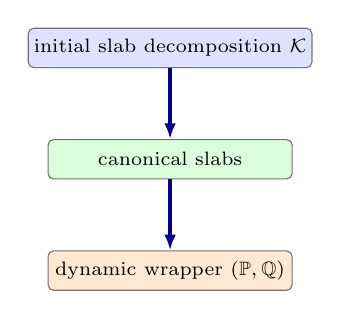
\begin{tikzpicture}[every node/.style={font=\scriptsize}]
\node[timeline,fill=blue!12,minimum width=3.1cm] (a) {initial slab decomposition $\cK$};
\node[timeline,fill=green!14,minimum width=3.1cm,below=0.9cm of a] (b) {canonical slabs};
\node[timeline,fill=orange!18,minimum width=3.1cm,below=0.9cm of b] (c) {dynamic wrapper $(\bbP,\bbQ)$};
\draw[flowarrow] (a) -- (b);
\draw[flowarrow] (b) -- (c);
\end{tikzpicture}

{\scriptsize Space is $\Oh_d(n)$ words, i.e. $\Oh_d(n\log n)$ bits on the word RAM.}
\end{columns}
\end{frame}

\begin{frame}[t]{What the proof stack actually needs}
\begin{columns}[T,totalwidth=\textwidth]
\column{0.55\textwidth}
\begin{enumerate}
\item A linear bound on the number of \emph{corners}.
\item A slab decomposition with only $\Oh_d(n)$ slabs.
\item A \emph{canonical} slab decomposition that can be recomputed efficiently.
\item A static point-location structure for those slabs.
\item A dynamic buffer of pending updates.
\end{enumerate}
\medskip
The algorithm never uses a contraction sequence directly after initialization: it exploits only structural consequences of bounded twin-orderedness.
\column{0.41\textwidth}
\centering
\DependencyGraphFig[0.95]
\end{columns}
\end{frame}

\begin{frame}[t]{Zones, corners, and slabs}
\begin{columns}[T,totalwidth=\textwidth]
\column{0.52\textwidth}
\begin{itemize}
\item A \emph{zone} is a submatrix $M[R,C]$ induced by a contiguous row block $R$ and a contiguous column block $C$.
\item A \emph{corner} is a $2\times 2$ zone whose two rows are different and whose two columns are different.
\item A \emph{slab} is a zone $M[[a,b],[c,d]]$ filled entirely with $1$-entries.
\end{itemize}
\begin{block}{Why slabs matter}
A slab decomposition is exactly a list of pairwise disjoint all-one rectangles covering every $1$ of the matrix.
\end{block}
\column{0.44\textwidth}
\centering
\ZoneCornerSlabFig[0.95]

{\scriptsize Blue frame: a zone. Thick black frame: a slab. Magenta cells witness a corner.}
\end{columns}
\end{frame}

\begin{frame}[t]{Example: a small slab decomposition}
\begin{columns}[T,totalwidth=\textwidth]
\column{0.48\textwidth}
\centering
\PrelimSlabFig[1.02]
\column{0.48\textwidth}
\begin{block}{This decomposition is}
\[
\cK={M[[1,1],[2,3]],\ M[[1,2],[5,5]],\ M[[3,3],[2,4]],\ M[[4,5],[1,3]],\ M[[4,5],[5,5]]}.
\]
\end{block}
\begin{itemize}
\item Slabs are pairwise disjoint.
\item Every $1$ lies in exactly one slab.
\item Dense rows or columns can still be described succinctly.
\end{itemize}
\end{columns}
\end{frame}
\begin{frame}[t]{Linear number of corners}
\begin{columns}[T,totalwidth=\textwidth]
\column{0.56\textwidth}
\begin{lemma}[Pilipczuk--Soko\l{}owski--Zych-Pawlewicz]
Let
\[
\fd=\frac{16}{3}(2d+3)^2 2^{4(2d+2)}.
\]
Any $d$-twin-ordered binary $n\times n$ matrix contains at most
\[
\fd,(n+2)\in\Oh_d(n)
\]
corners.
\end{lemma}
\medskip
This is the main structural input from the static compact-representation paper.
\column{0.38\textwidth}
\centering
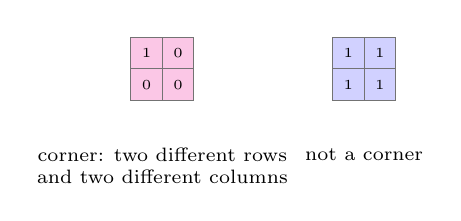
\begin{tikzpicture}[every node/.style={font=\scriptsize}]
\matrix[mini] (m) {
\CornerCell{1} \& \CornerCell{0}\\
\CornerCell{0} \& \CornerCell{0}\\
};
\node[below=0.35cm of m,font=\scriptsize,align=center] {corner: two different rows\\and two different columns};
\matrix[mini,right=1.5cm of m] (n) {
\Acell{1} \& \Acell{1}\\
\Acell{1} \& \Acell{1}\\
};
\node[below=0.35cm of n,font=\scriptsize,align=center] {not a corner};
\end{tikzpicture}
\vspace{2mm}

{\scriptsize The dynamic structure will only need the \emph{linear} bound, not its proof from contraction sequences.}
\end{columns}
\end{frame}

\begin{frame}[t]{Small slab decompositions exist}
\begin{columns}[T,totalwidth=\textwidth]
\column{0.58\textwidth}
\begin{lemma}[Pilipczuk--Soko\l{}owski--Zych-Pawlewicz]
Every $d$-twin-ordered $n\times n$ binary matrix admits a slab decomposition $\cK$ with
\[
|\cK|\le d(2n-2)+1.
\]
\end{lemma}
\begin{itemize}
\item This is the input format of $\mathtt{Init}(n,\cK)$.
\item The dynamic structure never stores the whole $n\times n$ matrix explicitly.
\item Later we replace an arbitrary small slab decomposition by a \emph{canonical} one.
\end{itemize}
\column{0.38\textwidth}
\centering
\PrelimSlabFig[0.96]
\end{columns}
\end{frame}

\begin{frame}[t]{Chan's static 2D orthogonal point location structure}
\begin{columns}[T,totalwidth=\textwidth]
\column{0.56\textwidth}
\begin{theorem}[Chan 2013]
Given $N$ pairwise disjoint slabs with coordinates in ${1,\dots,U}$, one can build a linear-space data structure that answers point-location queries in $\Oh(\log\log U)$ time, with preprocessing time $\Oh(N\log\log U)$.
\end{theorem}
\begin{block}{Role in our construction}
Once we have a slab decomposition of the current matrix, $(\mathtt{QueryBit}(i,j))$ becomes a point-location query for the point $(i,j)$.
\end{block}
\column{0.4\textwidth}
\centering
\PointLocationFig[0.92]
\end{columns}
\end{frame}

\begin{frame}[t]{The adhesive segment set: operations we need}
\begin{columns}[T,totalwidth=\textwidth]
\column{0.55\textwidth}
We maintain a dynamic set of pairwise disjoint, pairwise non-adjacent segments over ${1,\dots,n}$ and support:
\begin{itemize}
\item $\mathtt{Containing}([a,b])$,
\item $\mathtt{Adjacent}([a,b])$,
\item $\mathtt{Disjoint}([a,b])$,
\item $\mathtt{Merge}([a,b])$,
\item $\mathtt{Split}([a,b])$.
\end{itemize}
All operations run in worst-case time $\Oh(\log\log n)$ using $\Oh(n)$ memory.
\column{0.41\textwidth}
\centering
\SegmentExampleOne[0.9]

\vspace{2mm}
\SegmentExampleThree[0.9]
\end{columns}
\end{frame}

\begin{frame}[t]{Why the adhesive segment set is exactly the right primitive}
\begin{columns}[T,totalwidth=\textwidth]
\column{0.52\textwidth}
During the canonical-decomposition sweep, the current column $i$ is represented by the set $\strips_i$ of maximal all-one vertical segments.
\begin{itemize}
\item When a slab closes in column $i$, a segment must be removed from the current strips: use $\mathtt{Split}$.
\item When a slab opens in column $i+1$, a segment must be inserted and possibly glued to adjacent pieces: use $\mathtt{Merge}$.
\item To find which current strips may change, query ($\mathtt{Containing}$) and ($\mathtt{Adjacent}$).
\end{itemize}
\column{0.44\textwidth}
\centering
\SegmentExampleTwo[0.92]

\vspace{2mm}
\SegmentExampleFour[0.92]
\end{columns}
\end{frame}

\begin{frame}[t]{Canonical slab decomposition: start from column strips}
\begin{columns}[T,totalwidth=\textwidth]
\column{0.54\textwidth}
For each column $i$, an \emph{$i$-strip} is a slab $(a,b,i,i)$ such that it cannot be extended upward or downward inside column $i$.
\medskip

Equivalently, $[a,b]\in\strips_i$ iff the cells $(a,i),\dots,(b,i)$ are all $1$ and maximal with this property.
\begin{block}{Idea}
Canonical slabs are formed by gluing together identical strips that persist across consecutive columns.
\end{block}
\column{0.42\textwidth}
\centering
\StripsExampleFig[0.93]

{\scriptsize The blue and orange frames show two equal strips in consecutive columns.}
\end{columns}
\end{frame}

\begin{frame}[t]{Sibling strips and canonical slabs}
\begin{columns}[T,totalwidth=\textwidth]
\column{0.53\textwidth}
Strips $(a,b,i,i)\in\strips_i$ and $(a,b,j,j)\in\strips_j$ are \emph{siblings} if for every $k\in[i,j]$ the same strip $(a,b,k,k)$ belongs to $\strips_k$.
\medskip

Sibling is an equivalence relation on all strips. Each equivalence class, taken as a union over its columns, is a \emph{canonical slab}.
\begin{itemize}
\item every strip belongs to exactly one canonical slab;
\item the canonical slab decomposition is therefore unique.
\end{itemize}
\column{0.43\textwidth}
\centering
\CanonicalExampleTwo[0.98]

{\scriptsize Here the big yellow slab comes from one sibling class across columns $2$ and $3$.}
\end{columns}
\end{frame}

\begin{frame}[t]{Canonical versus arbitrary slab decompositions}
\begin{columns}[T,totalwidth=\textwidth]
\column{0.47\textwidth}
\centering
\CanonicalTwoCoarse[0.98]

{\scriptsize A non-canonical decomposition may use only two slabs.}
\column{0.49\textwidth}
\centering
\CanonicalExampleTwo[0.98]

{\scriptsize The canonical decomposition uses three slabs, because strips are glued only while their vertical extent stays identical.}
\end{columns}
\vspace{2mm}
\begin{block}{Why this extra rigidity helps}
The canonical decomposition reacts locally to openings and closings of strips; that is exactly what the sweep algorithm can maintain.
\end{block}
\end{frame}

\begin{frame}[t]{Canonical slabs are still few}
\begin{columns}[T,totalwidth=\textwidth]
\column{0.58\textwidth}
\begin{lemma}
If $\cR$ is the canonical slab decomposition of a $d$-twin-ordered $n\times n$ matrix, then
\[
|\cR|\le 4\fd(n+2)+4n\in\Oh_d(n).
\]
\end{lemma}
\begin{itemize}
\item Interior canonical slabs are charged to corners.
\item Boundary slabs account for the additive $4n$ term.
\item Each corner can intersect at most four pairwise disjoint canonical slabs.
\end{itemize}
\column{0.38\textwidth}
\centering
\CanonicalExampleOne[0.96]
\end{columns}
\end{frame}

\begin{frame}[t]{Charging interior canonical slabs to corners: setup}
\begin{columns}[T,totalwidth=\textwidth]
\column{0.56\textwidth}
Fix an interior canonical slab $(a,b,c,d)$ with
\[
1<a\le b<n,\qquad 1<c\le d<n.
\]
Look one column to the right:
\[
Z=M[[a,b],[d+1,d+1]].
\]
Since $(a,b,c,d)$ is canonical, the strip $(a,b,d+1,d+1)$ does \emph{not} belong to $\strips_{d+1}$.
\medskip

Three cases remain:
\begin{enumerate}
\item $Z$ is mixed;
\item $Z$ is all $1$;
\item $Z$ is all $0$.
\end{enumerate}
\column{0.4\textwidth}
\centering
\CornerMixedFig[1.05]
\end{columns}
\end{frame}
\begin{frame}[t]{Corner charging: case 1 --- the next column is mixed}
\begin{columns}[T,totalwidth=\textwidth]
\column{0.52\textwidth}
If $Z=M[[a,b],[d+1,d+1]]$ contains both $0$ and $1$, then the two-column zone
\[
M[[a,b],[d,d+1]]
\]
contains a corner intersecting $(a,b,c,d)$.
\medskip

Indeed, column $d$ is entirely $1$ on rows $a,\dots,b$, while column $d+1$ changes value somewhere inside the same row interval.
\begin{block}{Consequence}
A mixed next column immediately witnesses a corner touching the slab.
\end{block}
\column{0.44\textwidth}
\centering
\CornerMixedFig[1.18]
\end{columns}
\end{frame}

\begin{frame}[t]{Corner charging: cases 2 and 3}
\begin{columns}[T,totalwidth=\textwidth]
\column{0.49\textwidth}
\centering
\CornerOnesFig[1.1]

{\scriptsize If $Z$ is all $1$, then $(a,b,d+1,d+1)$ would be a strip unless the slab can be extended upward or downward, creating a corner near $(a-1,a)$ or $(b,b+1)$.}
\column{0.47\textwidth}
\centering
\CornerZerosFig[1.1]

{\scriptsize If $Z$ is all $0$, then both boundary $2\times2$ zones are corners.}
\end{columns}
\vspace{2mm}
Hence every interior canonical slab intersects a corner, and the linear bound follows.
\end{frame}

\begin{frame}[t]{The decomposition algorithm: statement and plan}
\begin{columns}[T,totalwidth=\textwidth]
\column{0.58\textwidth}
\begin{theorem}
There is an algorithm $\mathtt{Decompose}(n,\cK)$ that, given any slab decomposition $\cK$ of $M$, computes the canonical slab decomposition $\cR$ in time
\[
\Oh\bigl(n+|\cK|\log\log n\bigr).
\]
\end{theorem}
\begin{enumerate}
\item Compute opening sets $O_i$ and closing sets $C_i$.
\item Sweep left-to-right to compute $B_i=\strips_i\setminus\strips_{i+1}$.
\item Sweep right-to-left to compute $A_i=\strips_i\setminus\strips_{i-1}$.
\item Sweep once more to glue starts in $A_i$ to ends in $B_i$.
\end{enumerate}
\column{0.38\textwidth}
\centering
\SweepMatrixFig[1.0]
\end{columns}
\end{frame}

\begin{frame}[t]{Opening and closing sets $O_i$ and $C_i$}
\begin{columns}[T,totalwidth=\textwidth]
\column{0.54\textwidth}
For a given slab decomposition $\cK$ define
\[
O_i={[a,b]\mid (a,b,i,d)\in\cK\text{ for some }d\ge i},
\]
\[
C_i={[a,b]\mid (a,b,c,i)\in\cK\text{ for some }c\le i}.
\]
\begin{itemize}
\item $O_i$ stores vertical segments that \emph{open} at column $i$.
\item $C_i$ stores vertical segments that \emph{close} at column $i$.
\item They are extracted from $\cK$ in $\Oh(n+|\cK|)$ time.
\end{itemize}
\column{0.42\textwidth}
\centering
\SweepMatrixFig[0.95]

\vspace{1mm}
{\scriptsize For the 4-by-4 example: $O_1={[2,2],[4,4]}$, $O_2={[3,3]}$, $O_4={[1,1]}$.}
\end{columns}
\end{frame}

\begin{frame}[t]{Sweep example: the input matrix and its slabs}
\begin{columns}[T,totalwidth=\textwidth]
\column{0.44\textwidth}
\centering
\SweepMatrixFig[1.08]
\column{0.52\textwidth}
\begin{block}{Input decomposition}
\[
\cK={(2,2,1,3),\ (3,3,2,4),\ (4,4,1,4),\ (1,1,4,4)}.
\]
\end{block}
\begin{block}{Strips by column}
\begin{align*}
\strips_1&={[2,2],[4,4]},\\
\strips_2&={[2,4]},\\
\strips_3&={[2,4]},\\
\strips_4&={[1,1],[3,4]}.
\end{align*}
\end{block}
\end{columns}
\end{frame}

\begin{frame}[t]{Left-to-right sweep, round $i=1$}
\begin{columns}[T,totalwidth=\textwidth]
\column{0.46\textwidth}
\centering
\SweepMatrixFig[1.02]
\column{0.5\textwidth}
At the beginning, after merging all segments of $O_1$, the segment set stores
\[
\bbS=\strips_1={[2,2],[4,4]}.
\]
To move from column $1$ to column $2$:
\begin{itemize}
\item $C_1=\varnothing$,
\item $O_2={[3,3]}$.
\end{itemize}
Thus the potentially affected list is
\[
L_1={[2,2],[4,4]},
\]
and after $\mathtt{Merge}([3,3])$ we obtain
\[
\strips_2={[2,4]}.
\]
Hence
\[
B_1={[2,2],[4,4]}.
\]
\end{columns}
\end{frame}

\begin{frame}[t]{Left-to-right sweep, round $i=2$}
\begin{columns}[T,totalwidth=\textwidth]
\column{0.46\textwidth}
\centering
\SweepMatrixFig[1.02]
\column{0.5\textwidth}
Now the structure stores
\[
\bbS=\strips_2={[2,4]}.
\]
To move from column $2$ to column $3$:
\begin{itemize}
\item $C_2=\varnothing$,
\item $O_3=\varnothing$.
\end{itemize}
No strip is touched, so
\[
L_2=\varnothing,
\qquad
\strips_3={[2,4]},
\qquad
B_2=\varnothing.
\]
\begin{block}{Key point}
Columns $2$ and $3$ have identical maximal all-one segments, so the middle slab should continue across them.
\end{block}
\end{columns}
\end{frame}

\begin{frame}[t]{Left-to-right sweep, round $i=3$}
\begin{columns}[T,totalwidth=\textwidth]
\column{0.46\textwidth}
\centering
\SweepMatrixFig[1.02]
\column{0.5\textwidth}
Currently
\[
\bbS=\strips_3={[2,4]}.
\]
Now
\[
C_3={[2,2]},\qquad O_4={[1,1]}.
\]
Potentially affected strips are those
\begin{itemize}
\item containing $[2,2]$,
\item adjacent to $[1,1]$.
\end{itemize}
So
\[
L_3={[2,4]}.
\]
After splitting off $[2,2]$ and merging $[1,1]$, the stored set becomes
\[
\strips_4={[1,1],[3,4]},
\]
therefore
\[
B_3={[2,4]}.
\]
\end{columns}
\end{frame}

\begin{frame}[t]{Left-to-right sweep, round $i=4$}
\begin{columns}[T,totalwidth=\textwidth]
\column{0.46\textwidth}
\centering
\SweepMatrixFig[1.02]
\column{0.5\textwidth}
Finally
\[
\bbS=\strips_4={[1,1],[3,4]}.
\]
Since $\strips_5=\emptyset$, all current strips must end here.
\medskip

Indeed,
\[
C_4={[1,1],[3,3],[4,4]},\qquad O_5=\emptyset,
\]
so every remaining strip is affected and disappears. Consequently
\[
B_4={[1,1],[3,4]}.
\]
\begin{block}{Result of the left sweep}
\[
B_1={[2,2],[4,4]},\quad B_2=\varnothing,\quad B_3={[2,4]},\quad B_4={[1,1],[3,4]}.
\]
\end{block}
\end{columns}
\end{frame}
\begin{frame}[t]{From the two directional sweeps to the canonical slabs}
\begin{columns}[T,totalwidth=\textwidth]
\column{0.54\textwidth}
A symmetric right-to-left sweep computes
\[
A_i=\strips_i\setminus \strips_{i-1}.
\]
For the 4-by-4 example,
\[
A_1={[2,2],[4,4]},\quad A_2={[2,4]},\quad A_3=\varnothing,\quad A_4={[1,1],[3,4]}.
\]
\medskip

Each canonical slab starts with some $[a,b]\in A_c$ and ends with the same segment in some $B_d$.
\begin{block}{Invariant for the last sweep}
Store for each lower endpoint $a$ the current starting column of the slab that carries the segment $[a,b]$.
\end{block}
\column{0.42\textwidth}
\centering
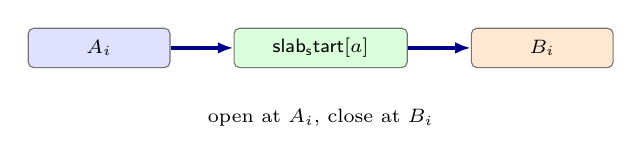
\begin{tikzpicture}[every node/.style={font=\scriptsize}]
\node[timeline,fill=blue!12,minimum width=1.8cm] (a1) {$A_i$};
\node[timeline,fill=green!14,minimum width=2.2cm,right=0.8cm of a1] (mid) {$\slabstart[a]$};
\node[timeline,fill=orange!18,minimum width=1.8cm,right=0.8cm of mid] (b1) {$B_i$};
\draw[flowarrow] (a1) -- (mid);
\draw[flowarrow] (mid) -- (b1);
\node[explain,below=0.4cm of mid] {open at $A_i$, close at $B_i$};
\end{tikzpicture}
\end{columns}
\end{frame}

\begin{frame}[t]{Final sweep on the example}
\begin{columns}[T,totalwidth=\textwidth]
\column{0.48\textwidth}
\begin{center}
\scriptsize
\begin{tabular}{c|c|c|c}
$i$ & $A_i$ & $B_i$ & slabs created in round $i$\\
\hline
$1$ & ${[2,2],[4,4]}$ & ${[2,2],[4,4]}$ & $(2,2,1,1),(4,4,1,1)$\\
$2$ & ${[2,4]}$ & $\varnothing$ & --\\
$3$ & $\varnothing$ & ${[2,4]}$ & $(2,4,2,3)$\\
$4$ & ${[1,1],[3,4]}$ & ${[1,1],[3,4]}$ & $(1,1,4,4),(3,4,4,4)$
\end{tabular}
\end{center}
\column{0.48\textwidth}
\centering
\SweepMatrixFig[1.08]

\vspace{2mm}
{\scriptsize The canonical decomposition is exactly
$(2,2,1,1),(4,4,1,1),(2,4,2,3),(1,1,4,4),(3,4,4,4)$.}
\end{columns}
\end{frame}

\begin{frame}[t]{Corollary: fast canonical decomposition of linear size}
\begin{columns}[T,totalwidth=\textwidth]
\column{0.58\textwidth}
\begin{corollary}
If $M$ is $d$-twin-ordered and $\cK$ is any slab decomposition of $M$, then $\mathtt{Decompose}(n,\cK)$ computes the canonical slab decomposition in time
\[
\Oh\bigl(n+|\cK|\log\log n\bigr)
\]
and the output contains at most
\[
4\fd(n+2)+4n\in\Oh_d(n)
\]
slabs.
\end{corollary}
\begin{itemize}
\item This is the structural engine behind the dynamic data structure.
\item The output size is linear in $n$ for fixed $d$.
\end{itemize}
\column{0.38\textwidth}
\centering
\CanonicalExampleOne[0.96]
\end{columns}
\end{frame}

\begin{frame}[t]{The amortized structure: two layers, one invariant}
\begin{columns}[T,totalwidth=\textwidth]
\column{0.56\textwidth}
The amortized data structure $\bbA$ stores:
\begin{enumerate}
\item a static point-location structure $\bbP$ on a canonical slab decomposition from some \emph{past} time;
\item a hash table $\bbQ$ of pending cell values that override $\bbP$.
\end{enumerate}
\begin{block}{Invariant}
If $(i,j)\in\bbQ$, then $M[i,j]=\bbQ[i,j]$.
Otherwise $M[i,j]=1$ iff $(i,j)$ lies in one of the slabs stored in $\bbP$.
\end{block}
\column{0.4\textwidth}
\centering
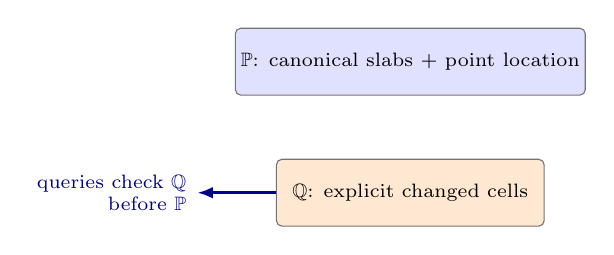
\begin{tikzpicture}[every node/.style={font=\scriptsize}]
\node[timeline,fill=blue!12,minimum width=3.4cm,minimum height=0.85cm] (p) {$\bbP$: canonical slabs + point location};
\node[timeline,fill=orange!18,minimum width=3.4cm,minimum height=0.85cm,below=0.8cm of p] (q) {$\bbQ$: explicit changed cells};
\draw[flowarrow] (q.west) -- ++(-1.0,0) node[left,align=right,font=\scriptsize] {queries check $\bbQ$\\before $\bbP$};
\end{tikzpicture}
\end{columns}
\end{frame}

\begin{frame}[t]{Initialization of the amortized structure}
\begin{columns}[T,totalwidth=\textwidth]
\column{0.58\textwidth}
\begin{enumerate}
\item Set $\bbQ\leftarrow\emptyset$.
\item Run $\mathtt{Decompose}(n,\cK)$ on the given slab decomposition.
\item Obtain the canonical output $\cR$ with
\[
|\cR|\le 4\fd(n+2)+4n.
\]
\item Build Chan's point-location structure $\bbP$ on $\cR$.
\end{enumerate}
\begin{block}{Cost}
\[
\Oh((n+|\cK|)\log\log n)
\]
expected time and $\Oh_d(n)$ space.
\end{block}
\column{0.38\textwidth}
\centering
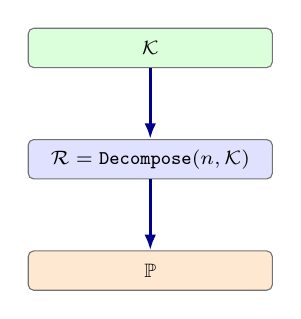
\begin{tikzpicture}[every node/.style={font=\scriptsize}]
\node[timeline,fill=green!14,minimum width=3.1cm] (a) {$\cK$};
\node[timeline,fill=blue!12,minimum width=3.1cm,below=0.9cm of a] (b) {$\cR=\mathtt{Decompose}(n,\cK)$};
\node[timeline,fill=orange!18,minimum width=3.1cm,below=0.9cm of b] (c) {$\bbP$};
\draw[flowarrow] (a) -- (b);
\draw[flowarrow] (b) -- (c);
\end{tikzpicture}
\end{columns}
\end{frame}

\begin{frame}[t]{QueryBit$(i,j)$}
\begin{columns}[T,totalwidth=\textwidth]
\column{0.55\textwidth}
\begin{enumerate}
\item Look up $(i,j)$ in $\bbQ$.
\item If present, return the stored value.
\item Otherwise issue a point-location query to $\bbP$.
\item Return $1$ iff $(i,j)$ lies in one of the stored slabs.
\end{enumerate}
\begin{block}{Complexity}
Hash-table lookup is expected $\Oh(1)$, point location is $\Oh(\log\log n)$, so
\[
\mathtt{QueryBit}(i,j)=\Oh(\log\log n)
\]
expected worst case.
\end{block}
\column{0.41\textwidth}
\centering
\PointLocationFig[0.93]
\end{columns}
\end{frame}

\begin{frame}[t]{Update$(i,j)$ before rebuilding}
\begin{columns}[T,totalwidth=\textwidth]
\column{0.56\textwidth}
\begin{enumerate}
\item If $(i,j)\in\bbQ$, negate the stored value.
\item Otherwise query $\bbP$ to obtain the current value.
\item Insert $(i,j)$ into $\bbQ$ with the negated result.
\end{enumerate}
\medskip
Thus $\bbQ$ stores the \emph{current value} of every touched cell since the last rebuild.
\begin{block}{Trigger}
When $|\bbQ|$ reaches
\[
L=8\fd(n+2),
\]
we rebuild $\bbP$ from scratch and reset $\bbQ$.
\end{block}
\column{0.4\textwidth}
\centering
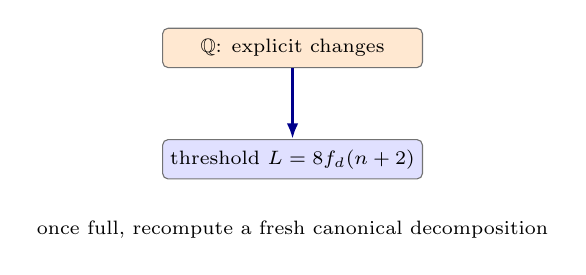
\begin{tikzpicture}[every node/.style={font=\scriptsize}]
\node[timeline,fill=orange!18,minimum width=3.3cm] (q0) {$\bbQ$: explicit changes};
\node[timeline,fill=blue!12,minimum width=3.3cm,below=0.9cm of q0] (thr) {threshold $L=8\fd(n+2)$};
\draw[flowarrow] (q0) -- (thr);
\node[explain,below=0.4cm of thr] {once full, recompute a fresh canonical decomposition};
\end{tikzpicture}
\end{columns}
\end{frame}

\begin{frame}[t]{Recomputing from $\bbP$ and $\bbQ$: the picture}
\begin{columns}[T,totalwidth=\textwidth]
\column{0.46\textwidth}
\centering
\AmortizedBaseFig[0.98]

{\scriptsize Left: slabs in $\cP$ with pending updates from $\cQ$ shown in bold.}
\column{0.5\textwidth}
\centering
\AmortizedAfterFig[0.98]

{\scriptsize Right: a fresh canonical decomposition of the up-to-date matrix.}
\end{columns}
\end{frame}

\begin{frame}[t]{Recomputing $\cK$: process all $0$-updates first}
\begin{columns}[T,totalwidth=\textwidth]
\column{0.56\textwidth}
Extract the list $\cQ$ from the hash table and partition it into
\begin{itemize}
\item $0$-updates, and
\item $1$-updates.
\end{itemize}
For every $0$-update, use $\bbP$ to identify the slab $P\in\cP$ that contains it.
\medskip

For each slab $P=(a,b,c,d)$, process the assigned updates row by row:
\begin{enumerate}
\item cut off the untouched prefix $P[<i]=(a,i-1,c,d)$,
\item isolate the row slab $P[i]=(i,i,c,d)$,
\item split that row slab around the $0$-updated columns,
\item continue with $P[>i]=(i+1,b,c,d)$.
\end{enumerate}
\column{0.4\textwidth}
\centering
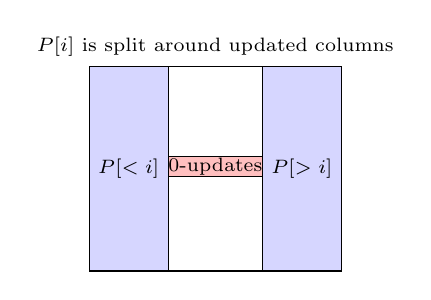
\begin{tikzpicture}[every node/.style={font=\scriptsize}]
\draw[fill=blue!16] (0,0) rectangle (3.2,2.6);
\draw[fill=white] (1.0,0) rectangle (2.2,2.6);
\draw[fill=red!25] (1.0,1.2) rectangle (2.2,1.45);
\node at (1.6,1.32) {$0$-updates};
\node at (0.5,1.3) {$P[<i]$};
\node at (2.7,1.3) {$P[>i]$};
\node at (1.6,2.85) {$P[i]$ is split around updated columns};
\end{tikzpicture}
\end{columns}
\end{frame}

\begin{frame}[t]{Recomputing $\cK$: then add the $1$-updates}
\begin{columns}[T,totalwidth=\textwidth]
\column{0.56\textwidth}
After processing all $0$-updates, each remaining $1$-update is handled independently:
\begin{itemize}
\item if the updated cell already belongs to some slab of $\cP$, ignore it;
\item otherwise add a $1\times 1$ slab for that cell.
\end{itemize}
\begin{block}{Size bound on the intermediate decomposition}
\[
|\cK|\le |\cP|+2|\cQ|.
\]
Indeed, every $0$-update increases the slab count by at most $2$, and every new $1$-update contributes at most one singleton slab.
\end{block}
\column{0.4\textwidth}
\centering
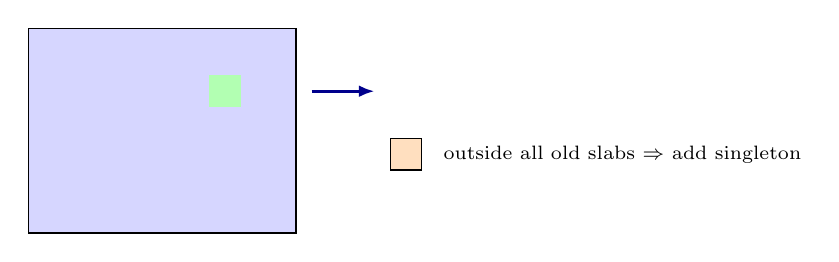
\begin{tikzpicture}[every node/.style={font=\scriptsize}]
\draw[fill=blue!16] (0,0) rectangle (3.4,2.6);
\fill[green!30] (2.3,1.6) rectangle +(0.4,0.4);
\draw[flowarrow] (3.6,1.8) -- (4.4,1.8);
\draw[fill=orange!25] (4.6,0.8) rectangle (5.0,1.2);
\node[align=left,anchor=west] at (5.15,1.0) {outside all old slabs $\Rightarrow$ add singleton};
\end{tikzpicture}
\end{columns}
\end{frame}

\begin{frame}[t]{Amortized theorem}
\begin{columns}[T,totalwidth=\textwidth]
\column{0.6\textwidth}
\begin{theorem}
The data structure $\bbA$ supports
\begin{itemize}
\item $\mathtt{Init}(n,\cK)$ in $\Oh((n+|\cK|)\log\log n)$ expected time,
\item $\mathtt{QueryBit}(i,j)$ in $\Oh(\log\log n)$ expected worst-case time,
\item $\mathtt{Update}(i,j)$ in $\Oh(\log\log n)$ expected amortized time,
\end{itemize}
using $\Oh_d(n)$ space.
\end{theorem}
Because rebuilding takes $\Oh(L\log\log n)$ total time and happens once every $L=8\fd(n+2)$ updates.
\column{0.36\textwidth}
\centering
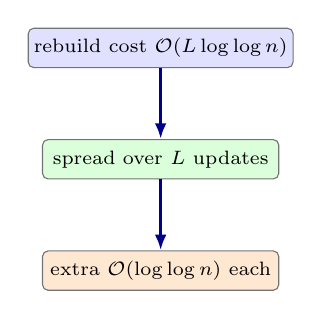
\begin{tikzpicture}[every node/.style={font=\scriptsize}]
\node[timeline,fill=blue!12,minimum width=3.0cm] (a) {rebuild cost $\Oh(L\log\log n)$};
\node[timeline,fill=green!14,minimum width=3.0cm,below=0.9cm of a] (b) {spread over $L$ updates};
\node[timeline,fill=orange!18,minimum width=3.0cm,below=0.9cm of b] (c) {extra $\Oh(\log\log n)$ each};
\draw[flowarrow] (a) -- (b);
\draw[flowarrow] (b) -- (c);
\end{tikzpicture}
\end{columns}
\end{frame}

\begin{frame}[t]{Why amortization is not enough}
\begin{columns}[T,totalwidth=\textwidth]
\column{0.56\textwidth}
For the main theorem we want \emph{expected worst-case} time per update, not only amortized time.
\medskip

A natural attempt is standard epoch-based rebuilding:
\begin{itemize}
\item partition updates into epochs of length $L$;
\item while one copy answers queries, build the next copy in the background;
\item in the next epoch let the new copy catch up.
\end{itemize}
This almost works --- but there is a subtle obstacle.
\column{0.4\textwidth}
\centering
\NaiveEpochFig[0.88]
\end{columns}
\end{frame}

\begin{frame}[t]{The subtle flaw in the naive de-amortization}
\begin{columns}[T,totalwidth=\textwidth]
\column{0.57\textwidth}
To initialize the next structure $\bbA_i$, we need the current slab list $\cK$ extracted from the previous structure $\bbA_{i-1}$.
\medskip

But extracting $\cK$ requires \emph{uninterrupted access} to the internal state of $\bbA_{i-1}$, while $\bbA_{i-1}$ must continue answering new updates during the same epoch.
\begin{block}{Conflict}
The builder wants a frozen snapshot; the live structure keeps mutating.
\end{block}
Without a snapshot, the new copy cannot even start its $\mathtt{Init}$ step safely.
\column{0.39\textwidth}
\centering
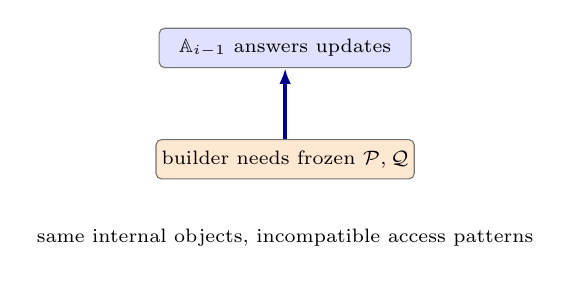
\begin{tikzpicture}[every node/.style={font=\scriptsize}]
\node[timeline,fill=blue!12,minimum width=3.2cm] (live) {$\bbA_{i-1}$ answers updates};
\node[timeline,fill=orange!18,minimum width=3.2cm,below=0.9cm of live] (need) {builder needs frozen $\cP,\cQ$};
\draw[flowarrow] (need) -- (live);
\node[explain,below=0.5cm of need] {same internal objects, incompatible access patterns};
\end{tikzpicture}
\end{columns}
\end{frame}

\begin{frame}[t]{The fix: two copies, one live and one snapshot}
\begin{columns}[T,totalwidth=\textwidth]
\column{0.56\textwidth}
For each epoch pair we keep two copies:
\[
\bbA_{i,0}\qquad\text{and}\qquad \bbA_{i,1}.
\]
Up to the beginning of epoch $E_{2i}$ they are initialized identically.
\medskip

At that point:
\begin{itemize}
\item $\bbA_{i,0}$ becomes the \emph{live} structure and processes new updates;
\item $\bbA_{i,1}$ stops changing and becomes a \emph{snapshot};
\item the next structure $\bbA_{i+1,*}$ is built from that snapshot.
\end{itemize}
\column{0.4\textwidth}
\centering
\SnapshotEpochFig[0.88]
\end{columns}
\end{frame}

\begin{frame}[t]{Final worst-case theorem and takeaways}
\begin{columns}[T,totalwidth=\textwidth]
\column{0.62\textwidth}
\begin{theorem}
There is a data structure $\bbW$ that maintains a dynamically updated $d$-twin-ordered $n\times n$ binary matrix using $\Oh_d(n)$ space and supports
\begin{itemize}
\item $\mathtt{Init}(n,\cK)$ in $\Oh((n+|\cK|)\log\log n)$ time,
\item $\mathtt{QueryBit}(i,j)$ in $\Oh(\log\log n)$ expected worst-case time,
\item $\mathtt{Update}(i,j)$ in $\Oh(\log\log n)$ expected worst-case time.
\end{itemize}
\end{theorem}
\begin{itemize}
\item Structural heart: canonical slabs of linear size.
\item Dynamic heart: a stale static structure plus a tiny update buffer.
\item Worst-case heart: the extra frozen copy.
\end{itemize}
\column{0.34\textwidth}
\centering
\DependencyGraphFig[0.88]
\end{columns}
\end{frame}

\appendix

\begin{frame}[t]{Backup guide}
\begin{columns}[T,totalwidth=\textwidth]
\column{0.58\textwidth}
The remaining slides provide:
\begin{itemize}
\item notation and example summaries;
\item more details on the adhesive segment set;
\item full corner-charging cases;
\item expanded sweep traces for $A_i,B_i$;
\item proof details for the amortized and worst-case structures;
\item open directions from the paper.
\end{itemize}
\column{0.38\textwidth}
\centering
\DependencyGraphFig[0.92]
\end{columns}
\end{frame}
\begin{frame}[t]{Notation cheat sheet}
\small
\begin{center}
\begin{tabular}{ll}
\toprule
Notation & meaning\\
\midrule
$M[i,j]$ & entry in row $i$, column $j$ of the current binary matrix\\
$M[R,C]$ & zone induced by a contiguous row block $R$ and column block $C$\\
$(a,b,c,d)$ & slab $M[[a,b],[c,d]]$ filled with ones\\
$\cK$ & an arbitrary slab decomposition of $M$\\
$\strips_i$ & maximal all-one segments in column $i$\\
$A_i$ & $\strips_i\setminus\strips_{i-1}$, strips that start at column $i$\\
$B_i$ & $\strips_i\setminus\strips_{i+1}$, strips that end at column $i$\\
$O_i$ & opening segments of slabs of $\cK$ at column $i$\\
$C_i$ & closing segments of slabs of $\cK$ at column $i$\\
$\bbS$ & adhesive segment set used inside the sweep\\
$\bbP$ & static point-location structure on canonical slabs\\
$\bbQ$ & hash table of pending updated cell values\\
$L$ & rebuild threshold $8\fd(n+2)$\\
\bottomrule
\end{tabular}
\end{center}
\end{frame}

\begin{frame}[t]{The contraction-sequence example at a glance}
\begin{columns}[T,totalwidth=\textwidth]
\column{0.32\textwidth}\centering
\ContractionStateOne[1.0]

\ContractionStateTwo[1.0]
\column{0.32\textwidth}\centering
\ContractionStateThree[1.0]

\ContractionStateFour[1.0]
\column{0.32\textwidth}\centering
\ContractionStateFive[1.0]

\ContractionStateSix[1.0]
\end{columns}
\vspace{2mm}
\begin{center}
\scriptsize These are the key intermediate states from the paper's width-$2$ contraction sequence illustration.
\end{center}
\end{frame}

\begin{frame}[t]{Tracking non-constant zones in the example}
\begin{columns}[T,totalwidth=\textwidth]
\column{0.47\textwidth}
\centering
\ContractionStateFour[1.18]
\column{0.49\textwidth}
\begin{itemize}
\item After merging rows $1$ and $2$, the upper middle block becomes non-constant.
\item The rightmost block of rows $3$ and $4$ is already non-constant.
\item The example is designed so that no row block and no column block ever sees more than two such blocks.
\end{itemize}
\begin{block}{Interpretation}
Twin-orderedness is a \emph{global regularity} condition: the matrix may be dense, but the inhomogeneity stays locally sparse with respect to the current block system.
\end{block}
\end{columns}
\end{frame}

\begin{frame}[t]{Corners: examples and non-examples}
\begin{columns}[T,totalwidth=\textwidth]
\column{0.3\textwidth}
\centering
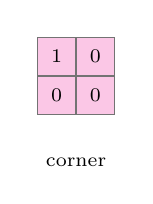
\begin{tikzpicture}[every node/.style={font=\scriptsize}]
\matrix[mat] (m) {
\CornerCell{1} \& \CornerCell{0}\\
\CornerCell{0} \& \CornerCell{0}\\
};
\node[below=0.3cm of m] {corner};
\end{tikzpicture}
\column{0.3\textwidth}
\centering
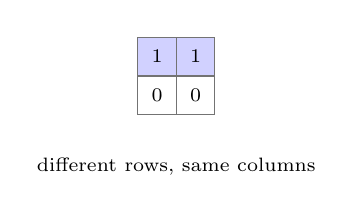
\begin{tikzpicture}[every node/.style={font=\scriptsize}]
\matrix[mat] (m) {
\Acell{1} \& \Acell{1}\\
\Zero{0} \& \Zero{0}\\
};
\node[below=0.3cm of m] {different rows, same columns};
\end{tikzpicture}
\column{0.34\textwidth}
\centering
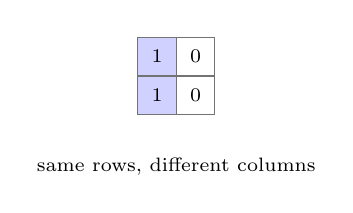
\begin{tikzpicture}[every node/.style={font=\scriptsize}]
\matrix[mat] (m) {
\Acell{1} \& \Zero{0}\\
\Acell{1} \& \Zero{0}\\
};
\node[below=0.3cm of m] {same rows, different columns};
\end{tikzpicture}
\end{columns}
\vspace{2mm}
A corner is the minimal obstruction to row-homogeneity and column-homogeneity simultaneously.
\end{frame}

\begin{frame}[t]{Why one corner can charge at most four canonical slabs}
\begin{columns}[T,totalwidth=\textwidth]
\column{0.54\textwidth}
A corner occupies a $2\times2$ area. Since slabs are pairwise disjoint rectangles of ones, at most one canonical slab can intersect each of the four cells adjacent to that corner.
\medskip

Therefore any charging argument from slabs to corners loses only a factor of $4$.
\column{0.42\textwidth}
\centering
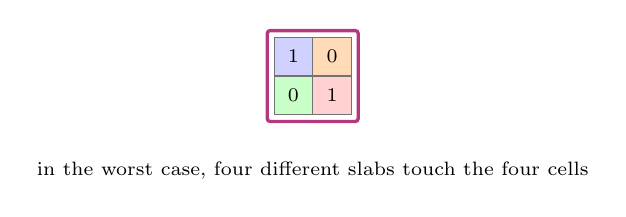
\begin{tikzpicture}[every node/.style={font=\scriptsize}]
\matrix[mat] (m) {
\Acell{1} \& \Bcell{0}\\
\Ccell{0} \& \Dcell{1}\\
};
\draw[very thick,magenta!70!black,rounded corners=1pt] ($(m-1-1.north west)+(-0.08,0.08)$) rectangle ($(m-2-2.south east)+(0.08,-0.08)$);
\node[below=0.35cm of m,align=center] {in the worst case, four different slabs touch the four cells};
\end{tikzpicture}
\end{columns}
\end{frame}

\begin{frame}[t]{How the small slab decomposition enters the story}
\begin{columns}[T,totalwidth=\textwidth]
\column{0.58\textwidth}
The dynamic structure assumes that the initial matrix is given as a slab decomposition $\cK$.
\medskip

The static representation result guarantees that, for every $d$-twin-ordered matrix, such a decomposition exists with only $\Oh_d(n)$ slabs and can be extracted from a contraction sequence.
\begin{block}{Why this matters}
Initialization does not need the entire dense matrix; it needs only a compressed geometric description of the $1$-entries.
\end{block}
\column{0.38\textwidth}
\centering
\PrelimSlabFig[0.94]
\end{columns}
\end{frame}

\begin{frame}[t]{Point location as a geometric query}
\begin{columns}[T,totalwidth=\textwidth]
\column{0.42\textwidth}
\centering
\PointLocationFig[1.0]
\column{0.54\textwidth}
Given disjoint slabs in the integer grid, point location asks:
\[
\text{which slab, if any, contains }(i,j)?
\]
\begin{itemize}
\item If some slab contains $(i,j)$, then $M[i,j]=1$.
\item Otherwise $M[i,j]=0$.
\end{itemize}
Because the slabs are disjoint, there is at most one positive answer.
\medskip

Chan's structure is the only nontrivial external black box in the paper.
\end{columns}
\end{frame}

\begin{frame}[t]{Adhesive segment set internals: a van Emde Boas dictionary on endpoints}
\begin{columns}[T,totalwidth=\textwidth]
\column{0.57\textwidth}
Store in a van Emde Boas dictionary $\bbD$ all endpoints of the maintained segments, together with one extra bit saying whether the endpoint is a start or an end.
\medskip

Then predecessor/successor queries in $\bbD$ let us recover:
\begin{itemize}
\item the segment containing a query interval;
\item the segments immediately adjacent to a query interval;
\item the appropriate endpoints to delete/insert during merges and splits.
\end{itemize}
\column{0.39\textwidth}
\centering
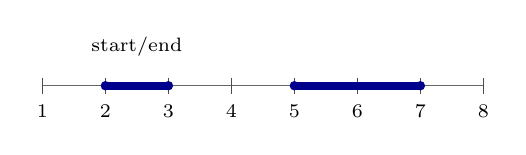
\begin{tikzpicture}[every node/.style={font=\scriptsize}]
\draw[black!60] (0,0) -- (5.6,0);
\foreach \x/\lab in {0/1,0.8/2,1.6/3,2.4/4,3.2/5,4.0/6,4.8/7,5.6/8} {
\draw[tick] (\x,0.1) -- (\x,-0.1);
\node[below] at (\x,-0.12) {\lab};
}
\fill[blue!55!black] (0.8,0) circle (0.06);
\fill[blue!55!black] (1.6,0) circle (0.06);
\fill[blue!55!black] (3.2,0) circle (0.06);
\fill[blue!55!black] (4.8,0) circle (0.06);
\node[above] at (1.2,0.25) {start/end};
\draw[segline] (0.8,0) -- (1.6,0);
\draw[segline] (3.2,0) -- (4.8,0);
\end{tikzpicture}
\end{columns}
\end{frame}

\begin{frame}[t]{Containing$([a,b])$ via predecessor and successor}
\begin{columns}[T,totalwidth=\textwidth]
\column{0.42\textwidth}
\centering
\SegmentExampleOne[1.0]
\column{0.54\textwidth}
To test whether $[a,b]$ is contained in some stored segment, query
\[
a'=\mathtt{Predecessor}(a+1),\qquad b'=\mathtt{Successor}(b-1).
\]
If $a'$ is the start of a segment, $b'$ is the corresponding end, and they match each other, then $[a,b]\subseteq[a',b']$.
\begin{block}{Why this is enough}
Since the maintained segments are pairwise disjoint and non-adjacent, the predecessor and successor around the query interval determine the unique candidate container.
\end{block}
\end{columns}
\end{frame}

\begin{frame}[t]{Adjacent$([a,b])$: find the at most two touching segments}
\begin{columns}[T,totalwidth=\textwidth]
\column{0.42\textwidth}
\centering
\SegmentExampleThree[1.0]
\column{0.54\textwidth}
A segment is adjacent to $[a,b]$ only if it contains $a-1$ or $b+1$.
\medskip

So the implementation reduces adjacency to two containing queries:
\[
\mathtt{Containing}([a-1,a-1]),\qquad \mathtt{Containing}([b+1,b+1]).
\]
\begin{itemize}
\item There can be at most one segment on the left.
\item There can be at most one segment on the right.
\end{itemize}
This is the operation used to discover which strips may merge with a newly opened vertical segment.
\end{columns}
\end{frame}

\begin{frame}[t]{Merge$([a,b])$: glue to adjacent segments if possible}
\begin{columns}[T,totalwidth=\textwidth]
\column{0.42\textwidth}
\centering
\SegmentExampleTwo[1.0]
\column{0.54\textwidth}
If $[a,b]$ is disjoint from all stored segments, there are three possibilities:
\begin{enumerate}
\item no adjacent segment $\Rightarrow$ insert $[a,b]$;
\item one adjacent segment $\Rightarrow$ replace it by the union;
\item two adjacent segments $\Rightarrow$ replace both by one larger segment.
\end{enumerate}
Predecessor/successor queries reveal the neighboring endpoints, so the update touches only $\Oh(1)$ dictionary keys.
\end{columns}
\end{frame}

\begin{frame}[t]{Split$([a,b])$: carve out a subsegment}
\begin{columns}[T,totalwidth=\textwidth]
\column{0.42\textwidth}
\centering
\SegmentExampleFour[1.0]
\column{0.54\textwidth}
If some stored segment $[a',b']$ contains $[a,b]$, then replace it by
\[
[a',a-1]\qquad\text{and}\qquad [b+1,b']
\]
whenever these segments are nonempty.
\medskip

During the canonical sweep this models the event that a slab closes in the current column and must be removed from the current strip set.
\end{columns}
\end{frame}

\begin{frame}[t]{Why the adhesive segment lemma has the advertised bounds}
\begin{columns}[T,totalwidth=\textwidth]
\column{0.58\textwidth}
\begin{itemize}
\item The dictionary universe is ${1,\dots,n}$, so each predecessor/successor search takes $\Oh(\log\log n)$ worst-case time.
\item Every high-level operation performs only a constant number of such searches and updates.
\item The extra bit telling whether an endpoint is a start or an end is stored in a static array of size $n$.
\end{itemize}
\begin{block}{Conclusion}
The adhesive segment set uses $\Oh(n)$ space and every operation runs in $\Oh(\log\log n)$ worst-case time.
\end{block}
\column{0.38\textwidth}
\centering
\SegmentExampleOne[0.9]

\vspace{1mm}
\SegmentExampleTwo[0.9]
\end{columns}
\end{frame}

\begin{frame}[t]{Another strips picture}
\begin{columns}[T,totalwidth=\textwidth]
\column{0.42\textwidth}
\centering
\StripsExampleFig[1.0]
\column{0.54\textwidth}
Read the columns separately:
\begin{itemize}
\item column $2$ has strips $[1,3]$ and $[5,5]$;
\item column $3$ has the same two strips;
\item column $4$ has only one strip $[3,5]$.
\end{itemize}
Hence the class of sibling strips across columns $2$ and $3$ forms one canonical slab, but it cannot continue into column $4$.
\end{columns}
\end{frame}

\begin{frame}[t]{Sibling relation really is an equivalence relation}
\begin{columns}[T,totalwidth=\textwidth]
\column{0.56\textwidth}
For strips of the form $(a,b,i,i)$, being siblings means that the same maximal vertical segment survives unchanged in every intermediate column.
\begin{itemize}
\item reflexive: every strip survives in its own column;
\item symmetric: the definition is symmetric in the two endpoints of the column interval;
\item transitive: if the same strip survives from $i$ to $j$ and from $j$ to $k$, it survives from $i$ to $k$.
\end{itemize}
Therefore canonical slabs are exactly the equivalence classes of strips.
\column{0.4\textwidth}
\centering
\CanonicalExampleTwo[0.96]
\end{columns}
\end{frame}
\begin{frame}[t]{Boundary slabs in the size lemma}
\begin{columns}[T,totalwidth=\textwidth]
\column{0.58\textwidth}
In the proof of the linear-size bound, only slabs with
\[
1<a\le b<n\qquad\text{and}\qquad 1<c\le d<n
\]
are charged to corners.
\medskip

Why? Because slabs touching the outer boundary of the matrix are not guaranteed to see a corner on the missing side.
\medskip

There are at most $4n$ such boundary slabs: one can charge them directly to a boundary row or boundary column.
\column{0.38\textwidth}
\centering
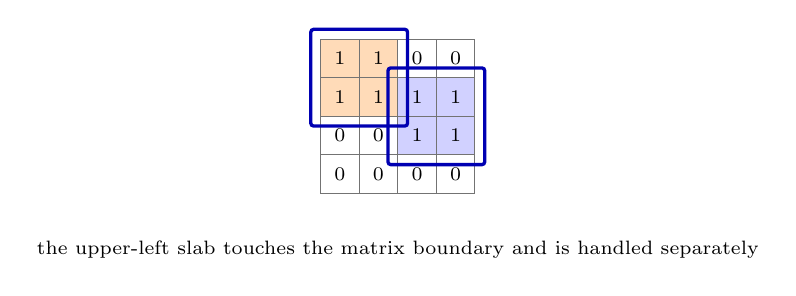
\begin{tikzpicture}[every node/.style={font=\scriptsize}]
\matrix[mat] (m) {
\Bcell{1} \& \Bcell{1} \& \Zero{0} \& \Zero{0}\\
\Bcell{1} \& \Bcell{1} \& \Acell{1} \& \Acell{1}\\
\Zero{0} \& \Zero{0} \& \Acell{1} \& \Acell{1}\\
\Zero{0} \& \Zero{0} \& \Zero{0} \& \Zero{0}\\
};
\node[zoneframe,fit=(m-1-1)(m-2-2)] {};
\node[zoneframe,fit=(m-2-3)(m-3-4)] {};
\node[below=0.35cm of m,align=center] {the upper-left slab touches the matrix boundary and is handled separately};
\end{tikzpicture}
\end{columns}
\end{frame}

\begin{frame}[t]{Interior slab setup for the charging argument}
\begin{columns}[T,totalwidth=\textwidth]
\column{0.56\textwidth}
Take an interior canonical slab $(a,b,c,d)$. By definition, $(a,b,d,d)$ is a strip, but $(a,b,d+1,d+1)$ is not.
\medskip

So the next column must witness some obstruction to continuing the same strip. That obstruction is converted into a nearby corner.
\begin{block}{Local view}
The proof only needs a constant-size neighborhood around the right boundary of the slab.
\end{block}
\column{0.4\textwidth}
\centering
\CornerMixedFig[1.08]
\end{columns}
\end{frame}

\begin{frame}[t]{Detailed case analysis: $Z$ is mixed}
\begin{columns}[T,totalwidth=\textwidth]
\column{0.56\textwidth}
If the next-column zone
\[
Z=M[[a,b],[d+1,d+1]]
\]
contains both $0$ and $1$, then in the two columns $d$ and $d+1$ there is a change inside rows $a,\dots,b$.
\medskip

Since column $d$ is entirely $1$ on that interval, the $2\times2$ submatrix around the change point is a corner.
\column{0.4\textwidth}
\centering
\CornerMixedFig[1.22]
\end{columns}
\end{frame}

\begin{frame}[t]{Detailed case analysis: $Z$ is all ones}
\begin{columns}[T,totalwidth=\textwidth]
\column{0.56\textwidth}
If $Z$ is all ones, then the obstruction is not horizontal --- it is vertical maximality.
\medskip

Because $(a,b,d+1,d+1)$ is not a strip, the all-one segment in column $d+1$ can be extended either above row $a$ or below row $b$.
\medskip

Comparing this with the strip in column $d$ yields a corner in either
\[
M[[a-1,a],[d,d+1]] \quad\text{or}\quad M[[b,b+1],[d,d+1]].
\]
\column{0.4\textwidth}
\centering
\CornerOnesFig[1.22]
\end{columns}
\end{frame}

\begin{frame}[t]{Detailed case analysis: $Z$ is all zeros}
\begin{columns}[T,totalwidth=\textwidth]
\column{0.56\textwidth}
If the next column is entirely zero on rows $a,\dots,b$, then the strip dies immediately on the right.
\medskip

Since column $d$ is entirely one on the same interval, both boundary $2\times2$ zones
\[
M[[a-1,a],[d,d+1]],\qquad M[[b,b+1],[d,d+1]]
\]
are corners.
\medskip

So in this easiest case the slab has two available witnesses.
\column{0.4\textwidth}
\centering
\CornerZerosFig[1.22]
\end{columns}
\end{frame}

\begin{frame}[t]{The sweep example: all opening and closing sets}
\begin{columns}[T,totalwidth=\textwidth]
\column{0.42\textwidth}
\centering
\SweepMatrixFig[1.06]
\column{0.54\textwidth}
\scriptsize
\begin{tabular}{c|c|c}
$i$ & $O_i$ & $C_i$\\
\hline
$1$ & ${[2,2],[4,4]}$ & $\varnothing$\\
$2$ & ${[3,3]}$ & $\varnothing$\\
$3$ & $\varnothing$ & ${[2,2]}$\\
$4$ & ${[1,1]}$ & ${[1,1],[3,3],[4,4]}$
\end{tabular}
\medskip

These are obtained directly from the input slabs:
\[
(2,2,1,3),\ (3,3,2,4),\ (4,4,1,4),\ (1,1,4,4).
\]
\end{columns}
\end{frame}

\begin{frame}[t]{Round $i=1$ in expanded detail}
\begin{columns}[T,totalwidth=\textwidth]
\column{0.45\textwidth}
\centering
\SweepMatrixFig[1.04]
\column{0.51\textwidth}
Start with $\bbS=\strips_1={[2,2],[4,4]}$.
\medskip

Since $C_1=\varnothing$, no split occurs. Since $O_2={[3,3]}$, the only operation is
\[
\mathtt{Merge}([3,3]).
\]
This merges the two adjacent current strips into the single segment $[2,4]$.
\medskip

Hence the two old strips disappear and exactly those belong to $B_1$.
\end{columns}
\end{frame}

\begin{frame}[t]{Round $i=2$ in expanded detail}
\begin{columns}[T,totalwidth=\textwidth]
\column{0.45\textwidth}
\centering
\SweepMatrixFig[1.04]
\column{0.51\textwidth}
Now $\bbS={[2,4]}$ and both $C_2$ and $O_3$ are empty.
\medskip

So the transition from column $2$ to column $3$ is structurally trivial:
\begin{itemize}
\item no strip disappears;
\item no new strip appears;
\item the current strip persists unchanged.
\end{itemize}
Consequently $B_2=\varnothing$.
\end{columns}
\end{frame}

\begin{frame}[t]{Round $i=3$ in expanded detail}
\begin{columns}[T,totalwidth=\textwidth]
\column{0.45\textwidth}
\centering
\SweepMatrixFig[1.04]
\column{0.51\textwidth}
The closing set $C_3={[2,2]}$ forces a split of the current strip $[2,4]$.
\medskip

The opening set $O_4={[1,1]}$ then inserts a new singleton strip adjacent to the upper remainder.
\medskip

After these two operations the current strip set becomes
\[
{[1,1],[3,4]},
\]
so the old segment $[2,4]$ is exactly the member of $B_3$.
\end{columns}
\end{frame}

\begin{frame}[t]{Round $i=4$ in expanded detail}
\begin{columns}[T,totalwidth=\textwidth]
\column{0.45\textwidth}
\centering
\SweepMatrixFig[1.04]
\column{0.51\textwidth}
At the last column every current strip must end, because $\strips_5=\emptyset$ by convention.
\medskip

The closing segments in $C_4$ remove both $[1,1]$ and $[3,4]$, and no opening segment is added afterwards.
\medskip

Therefore
\[
B_4={[1,1],[3,4]}.
\]
\end{columns}
\end{frame}

\begin{frame}[t]{Why the list $L_i$ is small}
\begin{columns}[T,totalwidth=\textwidth]
\column{0.58\textwidth}
In round $i$, the potentially affected list $L_i$ contains only
\begin{itemize}
\item strips containing some segment of $C_i$;
\item strips adjacent to some segment of $O_{i+1}$.
\end{itemize}
Each closing segment contributes at most one container, and each opening segment contributes at most two adjacent strips.
\begin{block}{Bound}
\[
|L_i|\le |C_i|+2|O_{i+1}|.
\]
\end{block}
After removing duplicates with a boolean table on lower endpoints, the whole round costs
\[
\Oh((|C_i|+|O_{i+1}|)\log\log n).
\]
\column{0.38\textwidth}
\centering
\SegmentExampleOne[0.9]

\vspace{1mm}
\SegmentExampleThree[0.9]
\end{columns}
\end{frame}

\begin{frame}[t]{Why $B_i$ is detected correctly}
\begin{columns}[T,totalwidth=\textwidth]
\column{0.58\textwidth}
Every strip in $\strips_i\setminus\strips_{i+1}$ must either
\begin{itemize}
\item contain a closing segment from $C_i$, or
\item be adjacent to an opening segment from $O_{i+1}$.
\end{itemize}
Otherwise it would survive unchanged from column $i$ to column $i+1$.
\medskip

So every disappearing strip is placed on the candidate list $L_i$. After performing the split/merge updates, we simply test whether each candidate is still present. Those that fail the test are exactly the members of $B_i$.
\column{0.38\textwidth}
\centering
\SweepMatrixFig[0.98]
\end{columns}
\end{frame}

\begin{frame}[t]{The right-to-left sweep for $A_i$}
\begin{columns}[T,totalwidth=\textwidth]
\column{0.58\textwidth}
The computation of
\[
A_i=\strips_i\setminus\strips_{i-1}
\]
is perfectly symmetric.
\medskip

Sweep from right to left, using closing segments on the left and opening segments on the previous column. The same adhesive segment-set operations and the same complexity analysis apply.
\begin{block}{For the 4-by-4 example}
\[
A_1={[2,2],[4,4]},\quad A_2={[2,4]},\quad A_3=\varnothing,\quad A_4={[1,1],[3,4]}.
\]
\end{block}
\column{0.38\textwidth}
\centering
\SweepMatrixFig[0.98]
\end{columns}
\end{frame}

\begin{frame}[t]{The final sweep with the array $\slabstart$}
\begin{columns}[T,totalwidth=\textwidth]
\column{0.52\textwidth}
Maintain an array $\slabstart[1..n]$ initialized with $\blank$.
\begin{itemize}
\item For every $(a,b)\in A_i$, set $\slabstart[a]=i$.
\item For every $(a,b)\in B_i$, output the slab
\[
(a,b,\slabstart[a],i).
\]
\end{itemize}
The index $a$ is enough because two different current strips never share the same lower endpoint.
\column{0.44\textwidth}
\centering
\scriptsize
\begin{tabular}{c|c|c}
$i$ & updates to $\slabstart$ & new slabs\\
\hline
$1$ & $\slabstart[2]=\slabstart[4]=1$ & $(2,2,1,1),(4,4,1,1)$\\
$2$ & $\slabstart[2]=2$ & --\\
$3$ & -- & $(2,4,2,3)$\\
$4$ & $\slabstart[1]=\slabstart[3]=4$ & $(1,1,4,4),(3,4,4,4)$
\end{tabular}
\end{columns}
\end{frame}

\begin{frame}[t]{Complexity summary for $\mathtt{Decompose}(n,\cK)$}
\begin{columns}[T,totalwidth=\textwidth]
\column{0.6\textwidth}
\begin{itemize}
\item Build all opening/closing buckets: $\Oh(n+|\cK|)$.
\item Left sweep for all $B_i$: $\Oh(n+|\cK|\log\log n)$.
\item Right sweep for all $A_i$: $\Oh(n+|\cK|\log\log n)$.
\item Final sweep with $\slabstart$: $\Oh(n+|\cK|)$.
\end{itemize}
Hence the total running time is
\[
\Oh(n+|\cK|\log\log n).
\]
\begin{block}{Output size}
By the corner bound, the canonical decomposition has at most $4\fd(n+2)+4n$ slabs.
\end{block}
\column{0.36\textwidth}
\centering
\DependencyGraphFig[0.85]
\end{columns}
\end{frame}
\begin{frame}[t]{Init on the running example}
\begin{columns}[T,totalwidth=\textwidth]
\column{0.44\textwidth}
\centering
\AmortizedBaseFig[0.95]
\column{0.52\textwidth}
Suppose the input decomposition $\cK$ describes the current matrix.
\medskip

Initialization performs:
\begin{enumerate}
\item $\bbQ\leftarrow\emptyset$;
\item compute the canonical decomposition $\cR=\mathtt{Decompose}(n,\cK)$;
\item build the point-location structure $\bbP$ on $\cR$.
\end{enumerate}
From then on, all future changes are buffered in $\bbQ$ until the rebuild threshold is hit.
\end{columns}
\end{frame}

\begin{frame}[t]{Why QueryBit is correct}
\begin{columns}[T,totalwidth=\textwidth]
\column{0.58\textwidth}
The correctness argument is exactly the invariant of the amortized structure.
\begin{itemize}
\item If $(i,j)\in\bbQ$, then by definition $\bbQ[i,j]$ stores the current value of the updated cell.
\item Otherwise the cell was untouched since the last rebuild, so its current value is exactly the value encoded by the slab decomposition inside $\bbP$.
\end{itemize}
\begin{block}{Therefore}
Checking $\bbQ$ first and $\bbP$ second always returns the current value $M[i,j]$.
\end{block}
\column{0.38\textwidth}
\centering
\PointLocationFig[0.9]
\end{columns}
\end{frame}

\begin{frame}[t]{Why Update preserves the invariant}
\begin{columns}[T,totalwidth=\textwidth]
\column{0.58\textwidth}
Two cases:
\begin{enumerate}
\item If $(i,j)\in\bbQ$, negate the stored value. Then $\bbQ[i,j]$ is again the current value.
\item If $(i,j)\notin\bbQ$, query $\bbP$ for the old value and insert its negation into $\bbQ$.
\end{enumerate}
No other cell changes, so the representation remains valid.
\medskip

When the threshold is reached, we rebuild and make $\bbP$ agree with the entire current matrix, after which $\bbQ$ can be emptied.
\column{0.38\textwidth}
\centering
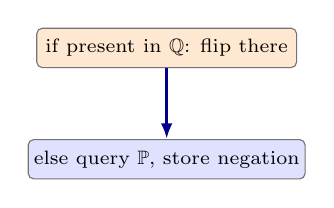
\begin{tikzpicture}[every node/.style={font=\scriptsize}]
\node[timeline,fill=orange!18,minimum width=3.3cm] (a) {if present in $\bbQ$: flip there};
\node[timeline,fill=blue!12,minimum width=3.3cm,below=0.9cm of a] (b) {else query $\bbP$, store negation};
\draw[flowarrow] (a) -- (b);
\end{tikzpicture}
\end{columns}
\end{frame}

\begin{frame}[t]{Assigning $0$-updates to old slabs}
\begin{columns}[T,totalwidth=\textwidth]
\column{0.44\textwidth}
\centering
\AmortizedBaseFig[0.95]
\column{0.52\textwidth}
Extract the pending updates from $\bbQ$ and sort them lexicographically.
\medskip

Every $0$-update must lie inside some old slab of $\cP$, because it changes a previously stored $1$ into a $0$.
\medskip

Using point location in $\bbP$, assign each such update to the slab that contains it. This yields, for every old slab $P\in\cP$, a sorted list $L_P$ of $0$-updates inside $P$.
\end{columns}
\end{frame}

\begin{frame}[t]{Process one slab row by row}
\begin{columns}[T,totalwidth=\textwidth]
\column{0.46\textwidth}
\centering
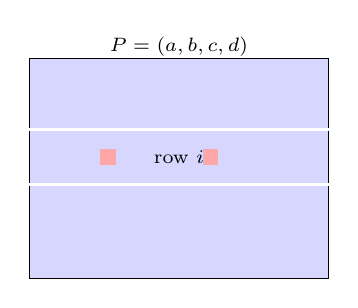
\begin{tikzpicture}[every node/.style={font=\scriptsize}]
\draw[fill=blue!16] (0,0) rectangle (3.8,2.8);
\draw[white,line width=1.2pt] (0,1.9) -- (3.8,1.9);
\draw[white,line width=1.2pt] (0,1.2) -- (3.8,1.2);
\fill[red!35] (0.9,1.45) rectangle +(0.2,0.2);
\fill[red!35] (2.2,1.45) rectangle +(0.2,0.2);
\node at (1.9,2.95) {$P=(a,b,c,d)$};
\node at (1.9,1.55) {row $i$};
\end{tikzpicture}
\column{0.5\textwidth}
For each row index $i$ that appears among the updates of $P$:
\begin{enumerate}
\item add the untouched prefix $P[<i]$ to the new decomposition;
\item isolate the one-row slab $P[i]$;
\item split $P[i]$ at the updated columns in that row;
\item continue recursively on the suffix $P[>i]$.
\end{enumerate}
This is exactly the procedure described in the proof of the amortized theorem.
\end{columns}
\end{frame}

\begin{frame}[t]{Within a single row slab: split around updated columns}
\begin{columns}[T,totalwidth=\textwidth]
\column{0.44\textwidth}
\centering
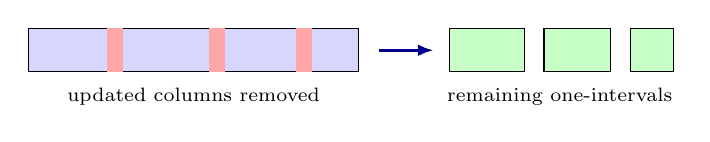
\begin{tikzpicture}[every node/.style={font=\scriptsize}]
\draw[fill=blue!16] (0,0) rectangle (4.2,0.55);
\fill[red!35] (1.0,0) rectangle +(0.2,0.55);
\fill[red!35] (2.3,0) rectangle +(0.2,0.55);
\fill[red!35] (3.4,0) rectangle +(0.2,0.55);
\draw[flowarrow] (4.45,0.27) -- (5.15,0.27);
\draw[fill=green!22] (5.35,0) rectangle +(0.95,0.55);
\draw[fill=green!22] (6.55,0) rectangle +(0.85,0.55);
\draw[fill=green!22] (7.65,0) rectangle +(0.55,0.55);
\node[below] at (2.1,-0.08) {updated columns removed};
\node[below] at (6.75,-0.08) {remaining one-intervals};
\end{tikzpicture}
\column{0.52\textwidth}
If $L_i={k_1<\dots<k_\ell}$ are the updated columns in row $i$, then the one-row slab is replaced by the intervals
\[
[c,k_1-1],\ [k_1+1,k_2-1],\ \dots,\ [k_\ell+1,d].
\]
Each nonempty interval becomes a new slab in $\cK$.
\medskip

The row contributes only $\Oh(|L_i|)$ new pieces.
\end{columns}
\end{frame}

\begin{frame}[t]{What happens with $1$-updates}
\begin{columns}[T,totalwidth=\textwidth]
\column{0.46\textwidth}
\centering
\AmortizedAfterFig[0.95]
\column{0.5\textwidth}
A $1$-update may already lie in an old slab of $\cP$; then it causes no change to the slab decomposition.
\medskip

Otherwise it is a genuinely new $1$-entry outside all old slabs, so we add a singleton slab for it.
\medskip

Later, when we run $\mathtt{Decompose}(n,\cK)$, such singleton slabs may merge into larger canonical slabs if neighboring strips coincide.
\end{columns}
\end{frame}

\begin{frame}[t]{Why $|\cK|\le |\cP|+2|\cQ|$}
\begin{columns}[T,totalwidth=\textwidth]
\column{0.58\textwidth}
Start with the old slab list $\cP$.
\begin{itemize}
\item Every $0$-update can increase the slab count by at most $2$: it removes one cell from a slab and thus creates at most two additional fragments.
\item Every $1$-update outside the old slabs creates at most one singleton slab.
\end{itemize}
Therefore the intermediate decomposition satisfies
\[
|\cK|\le |\cP|+2|\cQ|.
\]
Since both $|\cP|$ and $|\cQ|$ are $\Oh_d(n)$, rebuild remains linear-size.
\column{0.38\textwidth}
\centering
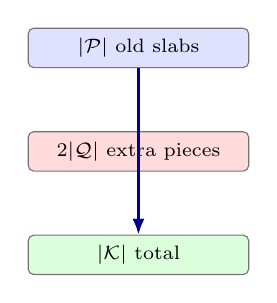
\begin{tikzpicture}[every node/.style={font=\scriptsize}]
\node[timeline,fill=blue!12,minimum width=2.8cm] (p) {$|\cP|$ old slabs};
\node[timeline,fill=red!14,minimum width=2.8cm,below=0.8cm of p] (q) {$2|\cQ|$ extra pieces};
\node[timeline,fill=green!14,minimum width=2.8cm,below=0.8cm of q] (k) {$|\cK|$ total};
\draw[flowarrow] (p) -- (k);
\draw[flowarrow] (q) -- (k);
\end{tikzpicture}
\end{columns}
\end{frame}

\begin{frame}[t]{Why each rebuild costs $\Oh(L\log\log n)$}
\begin{columns}[T,totalwidth=\textwidth]
\column{0.58\textwidth}
Recall the threshold
\[
L=8\fd(n+2).
\]
At rebuild time:
\begin{itemize}
\item $|\cQ|\le L$ by construction;
\item $|\cP|\le 4\fd(n+2)+4n=\Oh_d(n)$;
\item hence $|\cK|\le |\cP|+2|\cQ|=\Oh_d(n)=\Oh(L)$ for fixed $d$.
\end{itemize}
Running $\mathtt{Decompose}(n,\cK)$ and rebuilding Chan's structure both cost
\[
\Oh(L\log\log n).
\]
\column{0.38\textwidth}
\centering
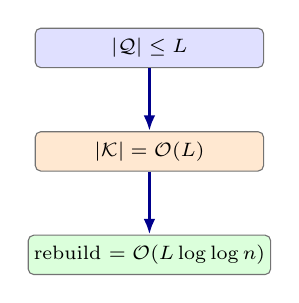
\begin{tikzpicture}[every node/.style={font=\scriptsize}]
\node[timeline,fill=blue!12,minimum width=2.9cm] (a) {$|\cQ|\le L$};
\node[timeline,fill=orange!18,minimum width=2.9cm,below=0.8cm of a] (b) {$|\cK|=\Oh(L)$};
\node[timeline,fill=green!14,minimum width=2.9cm,below=0.8cm of b] (c) {rebuild $=\Oh(L\log\log n)$};
\draw[flowarrow] (a) -- (b);
\draw[flowarrow] (b) -- (c);
\end{tikzpicture}
\end{columns}
\end{frame}

\begin{frame}[t]{Naive de-amortization: the epoch schedule}
\begin{columns}[T,totalwidth=\textwidth]
\column{0.42\textwidth}
\centering
\NaiveEpochFig[0.95]
\column{0.54\textwidth}
Let $E_0,E_1,E_2,\dots$ be epochs of length $L$.
\medskip

The intended plan is:
\begin{itemize}
\item structure $\bbA_i$ is initialized during epochs $E_{2i-2}$ and $E_{2i-1}$;
\item it answers queries during epochs $E_{2i}$ and $E_{2i+1}$.
\end{itemize}
At the end of the first build epoch, the new copy is one epoch behind; during the next epoch it processes two updates for every one live update and catches up.
\end{columns}
\end{frame}

\begin{frame}[t]{Catch-up during the odd epoch}
\begin{columns}[T,totalwidth=\textwidth]
\column{0.54\textwidth}
Suppose the new copy was initialized from the matrix state at the beginning of $E_{2i-2}$.
\medskip

After the build work is spread over all updates of $E_{2i-2}$, the new copy is exactly $L$ updates behind the live structure.
\medskip

During the next epoch $E_{2i-1}$, letting the new copy process \emph{two} buffered updates while the live copy processes one fresh update closes that gap by the end of the epoch.
\column{0.42\textwidth}
\centering
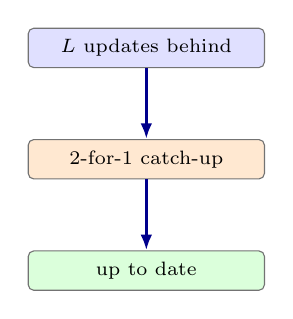
\begin{tikzpicture}[every node/.style={font=\scriptsize}]
\node[timeline,fill=blue!12,minimum width=3.0cm] (a) {$L$ updates behind};
\node[timeline,fill=orange!18,minimum width=3.0cm,below=0.9cm of a] (b) {2-for-1 catch-up};
\node[timeline,fill=green!14,minimum width=3.0cm,below=0.9cm of b] (c) {up to date};
\draw[flowarrow] (a) -- (b);
\draw[flowarrow] (b) -- (c);
\end{tikzpicture}
\end{columns}
\end{frame}

\begin{frame}[t]{Where uninterrupted access is needed}
\begin{columns}[T,totalwidth=\textwidth]
\column{0.56\textwidth}
The issue is not the catch-up phase. The issue is the very start of the build phase.
\medskip

To initialize the next copy, we need the current slab list $\cK$ obtained from the previous structure's internal data $(\cP,\cQ)$.
\medskip

Constructing that slab list takes linear time in its size and should see a consistent snapshot. A live structure that keeps updating cannot provide this consistency for free.
\column{0.4\textwidth}
\centering
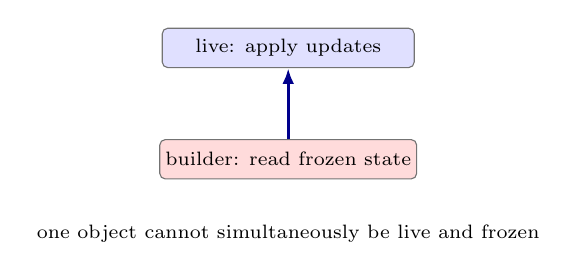
\begin{tikzpicture}[every node/.style={font=\scriptsize}]
\node[timeline,fill=blue!12,minimum width=3.2cm] (live) {live: apply updates};
\node[timeline,fill=red!14,minimum width=3.2cm,below=0.9cm of live] (snap) {builder: read frozen state};
\draw[flowarrow] (snap) -- (live);
\node[below=0.45cm of snap,align=center,font=\scriptsize] {one object cannot simultaneously be live and frozen};
\end{tikzpicture}
\end{columns}
\end{frame}

\begin{frame}[t]{Snapshot handoff in the corrected construction}
\begin{columns}[T,totalwidth=\textwidth]
\column{0.42\textwidth}
\centering
\SnapshotEpochFig[0.95]
\column{0.54\textwidth}
The corrected structure keeps two identical copies after initialization:
\[
\bbA_{i,0},\ \bbA_{i,1}.
\]
Once epoch $E_{2i}$ starts,
\begin{itemize}
\item $\bbA_{i,0}$ becomes live and continues processing all future updates;
\item $\bbA_{i,1}$ remains frozen and is handed to the builder of $\bbA_{i+1,*}$.
\end{itemize}
This resolves the consistency problem without changing asymptotic costs.
\end{columns}
\end{frame}
\begin{frame}[t]{Space bound after de-amortization}
\begin{columns}[T,totalwidth=\textwidth]
\column{0.58\textwidth}
At any moment, only a constant number of structures exist:
\begin{itemize}
\item one live copy,
\item one frozen snapshot of the same epoch,
\item one pair currently being built for the next epoch.
\end{itemize}
Each individual structure uses $\Oh_d(n)$ space, so multiplying by a constant preserves the bound.
\begin{block}{Conclusion}
The worst-case structure $\bbW$ still uses $\Oh_d(n)$ space.
\end{block}
\column{0.38\textwidth}
\centering
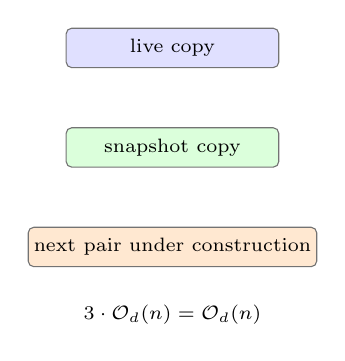
\begin{tikzpicture}[every node/.style={font=\scriptsize}]
\node[timeline,fill=blue!12,minimum width=2.7cm] (a) {live copy};
\node[timeline,fill=green!14,minimum width=2.7cm,below=0.75cm of a] (b) {snapshot copy};
\node[timeline,fill=orange!18,minimum width=2.7cm,below=0.75cm of b] (c) {next pair under construction};
\node[below=0.35cm of c,font=\scriptsize] {$3\cdot\Oh_d(n)=\Oh_d(n)$};
\end{tikzpicture}
\end{columns}
\end{frame}

\begin{frame}[t]{Why worst-case time stays $\Oh(\log\log n)$}
\begin{columns}[T,totalwidth=\textwidth]
\column{0.58\textwidth}
Every update performs only a constant number of actions:
\begin{itemize}
\item one update in the live structure,
\item a constant amount of scheduled rebuild work,
\item possibly a constant amount of catch-up work for the next structure.
\end{itemize}
Each action has expected cost $\Oh(\log\log n)$, so the overall expected worst-case time per update remains
\[
\Oh(\log\log n).
\]
\column{0.38\textwidth}
\centering
\begin{tikzpicture}[every node/.style={font=\scriptsize}]
\node[timeline,fill=blue!12,minimum width=3.0cm] (a) {live update};
\node[timeline,fill=orange!18,minimum width=3.0cm,below=0.8cm of a] (b) {scheduled build work};
\node[timeline,fill=green!14,minimum width=3.0cm,below=0.8cm of b] (c) {catch-up work};
\node[below=0.35cm of c,font=\scriptsize] {constant many $\times\ \Oh(\log\log n)$};
\end{tikzpicture}
\end{columns}
\end{frame}

\begin{frame}[t]{Dependency graph of the whole argument}
\begin{columns}[T,totalwidth=\textwidth]
\column{0.4\textwidth}
\centering
\DependencyGraphFig[1.0]
\column{0.56\textwidth}
\begin{enumerate}
\item Twin-orderedness gives a linear number of corners.
\item Corners imply linear-size canonical decompositions.
\item The sweep computes them quickly from any slab decomposition.
\item Chan turns canonical slabs into a fast static query structure.
\item Buffering updates gives amortized bounds.
\item Frozen copies de-amortize the construction.
\end{enumerate}
\end{columns}
\end{frame}

\begin{frame}[t]{Comparison with the static compact representation}
\begin{columns}[T,totalwidth=\textwidth]
\column{0.58\textwidth}
The static result of Pilipczuk, Soko\l{}owski, and Zych-Pawlewicz stores a $d$-twin-ordered matrix in $\Oh_d(n)$ \emph{bits} and answers queries in $\Oh_d(\log\log n)$ time.
\medskip

Our dynamic result stores the matrix in $\Oh_d(n)$ \emph{words} and supports both queries and updates in $\Oh(\log\log n)$ expected worst-case time.
\begin{block}{Tradeoff}
We gain dynamic updates, but we do not match the information-theoretic succinctness of the static representation.
\end{block}
\column{0.38\textwidth}
\centering
\begin{tikzpicture}[every node/.style={font=\scriptsize,align=center}]
\node[timeline,fill=blue!12,minimum width=2.8cm] (a) {static\\$\Oh_d(n)$ bits\\queries only};
\node[timeline,fill=orange!18,minimum width=2.8cm,below=1.0cm of a] (b) {dynamic\\$\Oh_d(n)$ words\\queries + updates};
\end{tikzpicture}
\end{columns}
\end{frame}

\begin{frame}[t]{Open direction 1: can the dynamic structure become succinct?}
\begin{columns}[T,totalwidth=\textwidth]
\column{0.58\textwidth}
The paper asks whether one can approach the static space bound while preserving fast updates.
\medskip

A target would be a dynamic representation using close to $\Oh_d(n)$ \emph{bits}, rather than $\Oh_d(n)$ words, with the same $\Oh(\log\log n)$ update/query complexity.
\begin{block}{Why this is hard}
The current design relies on geometric decompositions, hash tables, and explicit point-location structures --- all word-level objects.
\end{block}
\column{0.38\textwidth}
\centering
\begin{tikzpicture}[every node/.style={font=\scriptsize}]
\node[timeline,fill=blue!12,minimum width=3.0cm] (a) {$\Oh_d(n)$ bits?};
\node[timeline,fill=orange!18,minimum width=3.0cm,below=0.9cm of a] (b) {dynamic + succinct};
\draw[flowarrow] (a) -- (b);
\end{tikzpicture}
\end{columns}
\end{frame}

\begin{frame}[t]{Open direction 2: efficient submatrix flips}
\begin{columns}[T,totalwidth=\textwidth]
\column{0.52\textwidth}
A natural extension is to support an update that flips all bits in a whole zone $M[R,C]$.
\medskip

Such an operation is much more structured than arbitrary cell updates, but it also correlates many changes at once.
\begin{block}{Challenge}
The current update buffer $\bbQ$ is cell-based. A region flip would need a more expressive summary while preserving fast rebuilds.
\end{block}
\column{0.44\textwidth}
\centering
\begin{tikzpicture}[every node/.style={font=\scriptsize}]
\matrix[mat] (m) {
\Zero{0} \& \Zero{0} \& \Zero{0} \& \Zero{0}\\
\Zero{0} \& \Acell{1} \& \Acell{1} \& \Zero{0}\\
\Zero{0} \& \Acell{1} \& \Acell{1} \& \Zero{0}\\
\Zero{0} \& \Zero{0} \& \Zero{0} \& \Zero{0}\\
};
\node[zoneframe,fit=(m-2-2)(m-3-3)] {};
\node[below=0.35cm of m,align=center] {flip an entire zone instead of one cell};
\end{tikzpicture}
\end{columns}
\end{frame}

\begin{frame}[t]{Open direction 3: dynamic contraction sequences}
\begin{columns}[T,totalwidth=\textwidth]
\column{0.58\textwidth}
The current result assumes only that the matrix always stays $d$-twin-ordered. It does \emph{not} maintain any contraction sequence dynamically.
\medskip

A dynamic analogue of the greedy contraction-sequence construction from the twin-width literature could be useful far beyond matrix representation.
\begin{block}{Potential payoff}
Dynamic maintenance of contraction sequences could enable dynamic versions of other twin-width algorithms, such as first-order model checking or optimization problems on bounded-twin-width classes.
\end{block}
\column{0.38\textwidth}
\centering
\ContractionStateSix[1.05]
\end{columns}
\end{frame}

\begin{frame}[t]{Another canonical decomposition example from the paper}
\begin{columns}[T,totalwidth=\textwidth]
\column{0.46\textwidth}
\centering
\CanonicalExampleOne[1.0]
\column{0.5\textwidth}
This example is useful to keep in mind during questions:
\begin{itemize}
\item the long gray slab in column $2$ is vertical and maximal;
\item the red slab in the upper-right corner is created by sibling strips across columns $4$ and $5$;
\item the yellow slab in the fourth row cannot extend upward because column $3$ changes shape.
\end{itemize}
It shows how canonical slabs are constrained simultaneously by vertical maximality and horizontal persistence.
\end{columns}
\end{frame}

\begin{frame}[t]{Main constants and thresholds}
\small
\begin{center}
\begin{tabular}{ll}
\toprule
quantity & exact expression / role\\
\midrule
$\fd$ & $\frac{16}{3}(2d+3)^2 2^{4(2d+2)}$ from the corner bound\\
number of corners & at most $\fd(n+2)$\\
canonical slab count & at most $4\fd(n+2)+4n$\\
rebuild threshold $L$ & $8\fd(n+2)$ pending updates\\
$\mathtt{Decompose}$ time & $\Oh(n+|\cK|\log\log n)$\\
Chan preprocessing & $\Oh(N\log\log n)$ for $N$ slabs\\
query time & $\Oh(\log\log n)$ expected worst case\\
update time & $\Oh(\log\log n)$ amortized, then de-amortized to worst case\\
space & $\Oh_d(n)$ words\\
\bottomrule
\end{tabular}
\end{center}
\end{frame}

\begin{frame}[t]{Selected references}
\footnotesize
\begin{thebibliography}{9}
\bibitem{tww1}
'{E}. Bonnet, E. J. Kim, S. Thomass'e, and R. Watrigant.
\newblock Twin-width I: Tractable FO Model Checking.
\newblock \emph{Journal of the ACM}, 69(1), 2022.

\bibitem{repr}
M. Pilipczuk, M. Soko\l{}owski, and A. Zych-Pawlewicz.
\newblock Compact Representation for Matrices of Bounded Twin-Width.
\newblock In \emph{STACS 2022}.

\bibitem{chan}
T. M. Chan.
\newblock Persistent Predecessor Search and Orthogonal Point Location on the Word RAM.
\newblock \emph{ACM Transactions on Algorithms}, 9(3), 2013.

\bibitem{veb}
P. van Emde Boas.
\newblock Preserving order in a forest in less than logarithmic time and linear space.
\newblock \emph{Information Processing Letters}, 6(3), 1977.
\end{thebibliography}
\end{frame}

\begin{frame}[t]{One-page proof map}
\begin{columns}[T,totalwidth=\textwidth]
\column{0.44\textwidth}
\centering
\DependencyGraphFig[1.0]
\column{0.52\textwidth}
\begin{enumerate}
\item $d$-twin-ordered $\Rightarrow$ only linearly many corners.
\item Corners $\Rightarrow$ only linearly many canonical slabs.
\item Adhesive-segment sweeps compute those slabs in near-linear time.
\item Chan answers point queries on the static canonical decomposition.
\item Buffer updates in a small hash table and rebuild at threshold $L$.
\item Freeze one copy to de-amortize rebuilds.
\end{enumerate}
This is the entire architecture of the paper on one slide.
\end{columns}
\end{frame}

\begin{frame}[t]{Cheat sheet for questions}
\small
\begin{itemize}
\item \textbf{Input promise:} the row/column order is fixed, and the matrix remains $d$-twin-ordered after every flip.
\item \textbf{Static geometric object:} the canonical slab decomposition of size $\Oh_d(n)$.
\item \textbf{Dynamic invariant:} current values are encoded by a stale canonical decomposition $\bbP$ plus a small explicit override table $\bbQ$.
\item \textbf{Rebuild mechanism:} recover an intermediate slab decomposition from old slabs and buffered updates, then run $\mathtt{Decompose}$ again.
\item \textbf{Worst-case fix:} maintain a frozen snapshot copy for the next builder.
\end{itemize}
\vfill
\begin{center}
\Large Thank you.
\end{center}
\end{frame}

\end{document}
